%!TEX program = xelatex
\documentclass[a4paper]{ctexart}

\usepackage{listings} 
\usepackage{geometry}
\usepackage{booktabs}
\usepackage{graphicx}
\usepackage{tabularx}
\usepackage{multirow}
\usepackage{enumitem}
\usepackage{url}
\usepackage{ulem}
\usepackage{placeins}
\usepackage[bottom]{footmisc}

\renewcommand{\multirowsetup}{\centering}

\geometry{
    left=23mm,
    right=23mm,
    top=23mm,
    bottom=23mm,
}

\setlength{\parskip}{0.5em}

\title{\Huge PetLover 商业模式评估文档}

\author{
  项目成员:\\
  姬筠刚 191250055(PM)\\
  陈梓俊 191250016\\
  丁炳智 191250024\\
  刘庭烽 191250093\\
}
\date{\today}

\begin{document}

\maketitle

\centerline{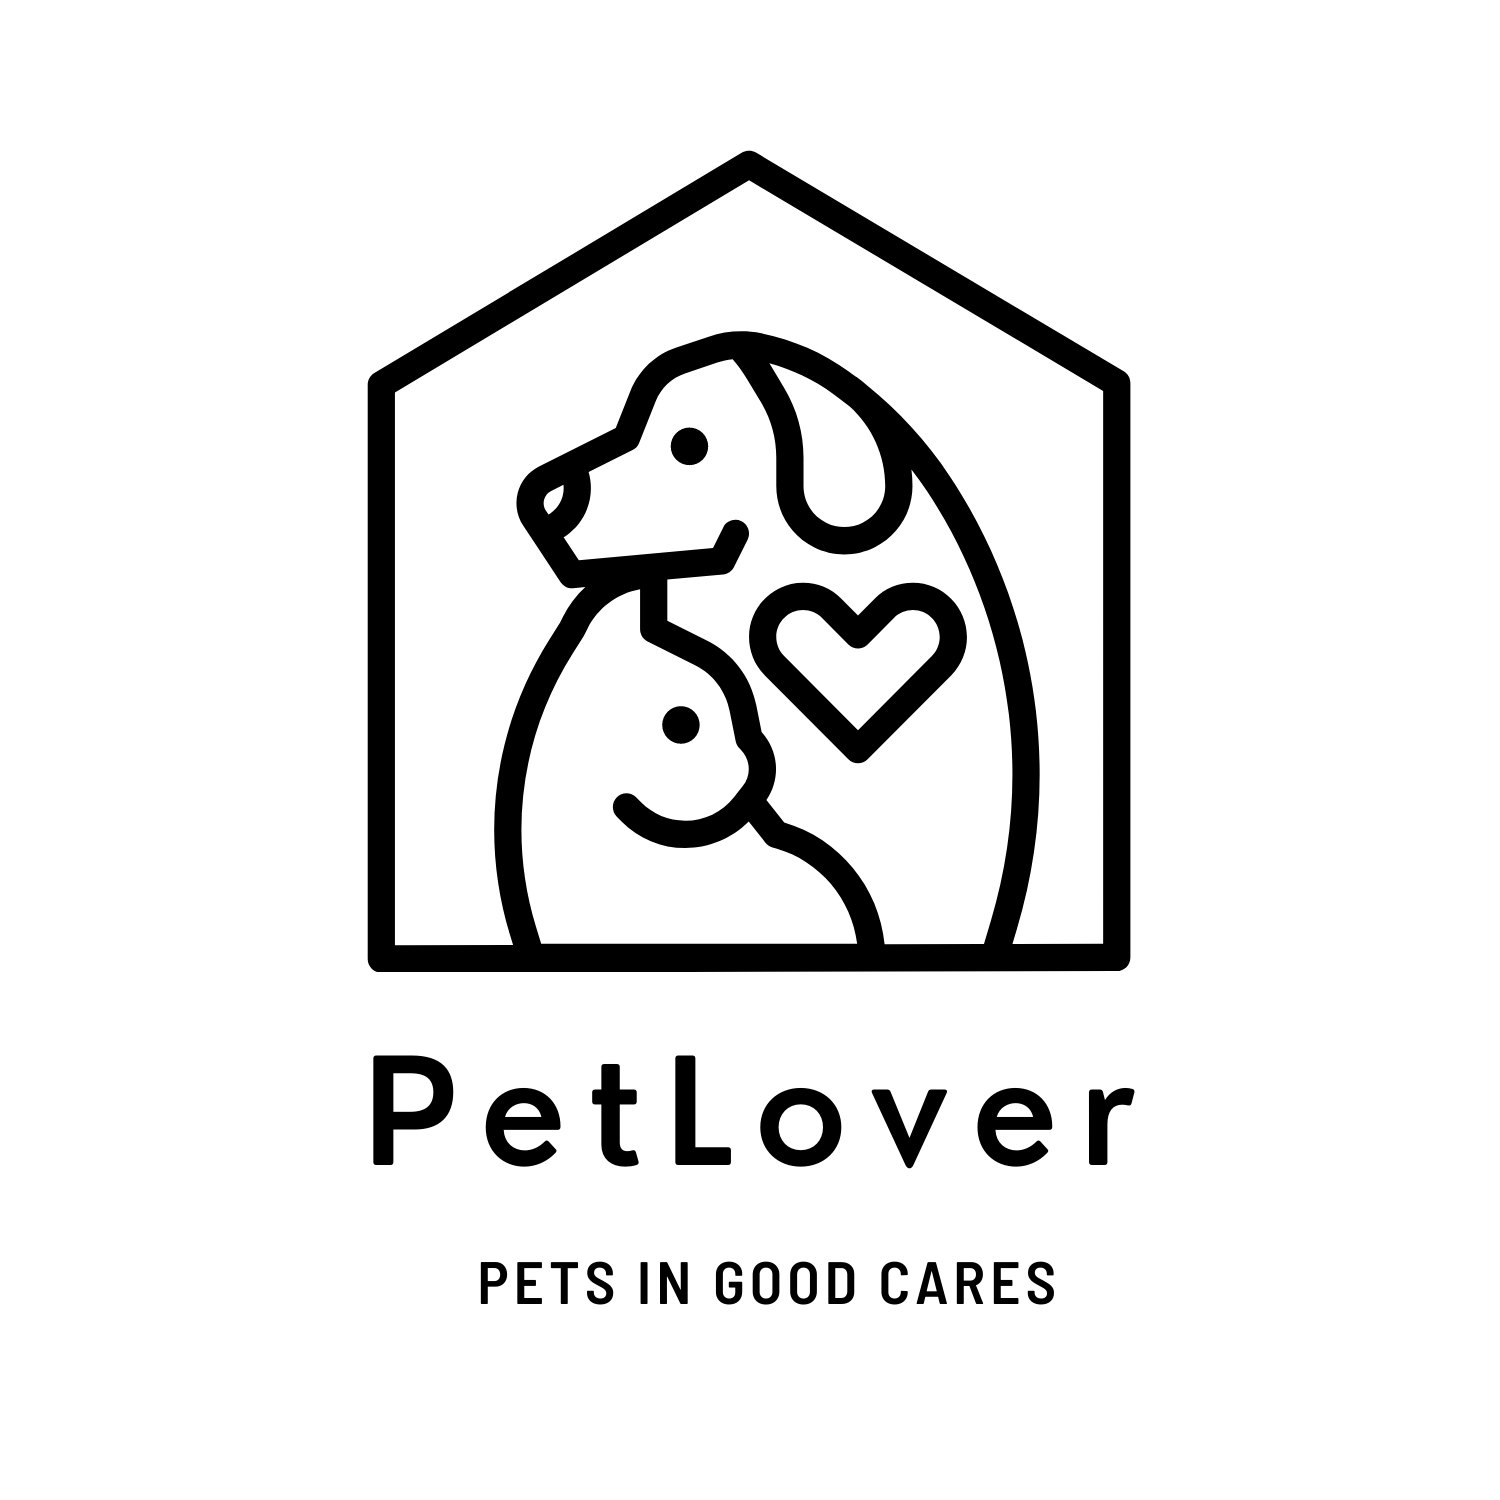
\includegraphics[]{logo.png}}

\newpage

\begin{abstract}
  本项目名为PetLover,是由本小组于2021年秋季学期《需求与商业模式创新》课程大作业中设计的软件产品项目。此文档为商业模式评估文档,主要内容包含本项目的商业模式评估有关的三种评估方式(包括商业模式环境、评估商业模式、蓝海战略)以及根据评估结果给出的更新过的商业模式画布。
\end{abstract}

\tableofcontents

\newpage

\setlength{\parskip}{1em}

\section{总览}
\subsection{工作概要}
本阶段是商业模式评估阶段,我们综合项目启动和商业模式设计两个阶段的成果,使用商业模式评估的方法重新对PetLover的商业模式进行审视,我们从商业模式环境、评估商业模式、蓝海战略三个方向入手。首先每个人分别对在市场影响力(五个子方向)、行业影响力(五个子方向)、关键趋势(四个子方向)和宏观经济影响(四个子方向)方面四个方面对PetLover的商业模式进行外部环境评估;然后我们通过讨论对商业模式进行了总体评估,使用SWOT方法从多方面对PetLover商业模式进行优势、劣势、机会、威胁的评估,同时思考增加优势,改善劣势的创意。最后我们汇总了所有成员的创意,选出了最适合的一个创意在价值主张方向的蓝海战略,汇总和筛选先前的所有分析与评估,用于更新商业模式画布。

\subsection{内容框架}
在商业模式环境板块中,我们从多方搜集资料,从不同的角度对我们商业模式的目标环境进行分析与阐释。在商业模式评估板块中,我们按照书上的条目,逐一对照,对我们的商业模式进行打分,并给出响应的分析或者理由。在蓝海战略板块中,我们遵循“删除、削减、增加、创造”的格式来描写我们的解决方案,并画出画布上的改变给出更直观的阐释。在画布更新板块中,我们给出了最终决定的更新后的画布,并阐述了更新的要点内容以及其所引起的画布的要点和关系上的改变逻辑。

\subsection{度量数值}
教材上列举的商业模式环境里每个方面的每个子问题下的所有主要问题都与PetLover的商业模式结合,然后进行回答;总体评估中的加分项为6项,减分项有3项,总体达到9项;SWOT 分析(包含机会与威胁评估)中的所有评分项都已经打分并阐述理由。整个三阶段作业所引用的调研报告和新闻达到36 篇。更新过的商业模式画布中新增或修改过的模块要点数量为8项,没有超过二阶段画布模块要点总数(41项)的30\%,并指出了发生变化的元素与元素之间的依赖关系(4条)。

\section{商业模式环境}
\subsection{市场影响力}
\subsubsection{市场问题}
\begin{enumerate}[label=\alph*.]
  \item 问题:影响客户环境的关键问题有哪些?哪些变化正在发生?市场朝向什么方向发展?
  \paragraph{解读:}宠物市场和相关社区论坛近些年正在发生哪些变化?宠物市场会向什么样的方向发展?
  \paragraph{回答:}探究所处市场和竞品的发展趋势和方向是PetLover团队思考自身产品优势劣势、机会威胁的关键所在。我国经济的快速发展,带动了不少行业,宠物业拥有着庞大的市场,养宠人士每年不断的增加,可以确定这个行业的未来是不可估量的;为了迎合用户需求,各种宠物软件层出不穷,例如爱宠市场、爱宠大陆等等,宠物弃养、宠物健康、虐待宠物等等一些宠物乱象成为近些年来的热点话题;另外社会调研报告发现,90后成为养宠人群中的主要群体,北上广深等一、二线城市成为养宠群体聚集地。可以预测未来宠物市场发展将会整合宠物医疗服务、宠物生活服务、宠物网络社区为一体,为现在还在跨平台的用户提供极大的便利,并在这三项服务上做到可靠、优质,另外随着养宠群体的不断扩大,宠物市场在“互联网+”时代很有可能从各大综合平台(如微博超话、Bilibili动物圈等)独立出来成为一个崭新的平台,而不单单作为一个子平台存在。PetLover迎合当今的宠物市场的变化,推出以一站式服务的为价值主张的平台,让用户体验更加良好!
  \paragraph{依据:}1、《网络社区营销策略和未来!》\\(https://zhuanlan.zhihu.com/p/314023382)\\
  本文讲到在我们的网络推广过程当中,社区是一个相当重要的渠道。拿小红书作为例子,发布内容回答「买什么」、「哪里买」、「多少钱」三个问题、推荐部分会将笔记分门别类,美妆、家具、健身、美食、读书、数码、汽车、音乐等等很多内容,极大方便了各类用户群体。网络社区有能力成为一个真正意义上的聚会的场所,在大多数情况下,可以取代人们在现实生活中的聚会场所。
  \item 问题:影响客户环境的关键问题有哪些?
  \paragraph{解读:}宠物社区及宠物市场受哪些关键问题的影响?
  \paragraph{回答:}网络社区存在并持续发展的关键是流量,流量的关键是吸引客户,我们的商业模式关键业务有爱宠社区和商品买卖,所以探究影响客户环境的关键问题非常重要。第一,提供优质的社区论坛服务需要优质内容支撑,客户往往为了准确且实用的回答和内容而绞尽脑汁,平台保证自身内容的质量才能留住客户;第二,平台宠物商品买卖受商品性价比和可靠性影响;第三,宠物商品买卖和社区论坛的操作便利性也是影响宠物社区和市场关键问题。目前的宠物相关市场环境不能很好地解决以上这三个问题,因此解决这些问题是我们的市场定位。
  \paragraph{依据:}1、《2020年中国宠物行业白皮书:超六成宠主已具备科学养宠意识》\\
  (https://blog.csdn.net/qadnmcrfxcn6c6h6661/article/details/113285471)\\
  中国宠物行业白皮书通过数据描绘宠主画像,对覆盖产业链上中下游全链路市场进行深入研究,全面解读中国宠物行业最新态势,为行业发展提供全新思考与实践方向。文章针对宠物市场提出了以下两点发展态势:宠物健康备受瞩目、推动宠主教育是推动科学养宠的关键。\\
  2、《宠物行业发展现状分析:宠物app是新的红海吗?》\\(http://www.woshipm.com/evaluating/4039367.html)\\
  本文着重分析2018-2019年来的宠物行业数据,宠物APP发展情况,以行业数据搭配宠物业内公司的3847份有效问卷调查加以客观分析。文章根据市场现状及发展趋势对宠物APP发展的可行性、食品消费洞察、消费渠道偏好进行了调研,提出近期宠物市场也是存在着惊人的活力,所以无论是全方位或是垂直领域下的宠物app,都应抓住本质需求精神慰藉,集中核心功能点的完善,再进行发散的观点。\\
  3、2021宠物医院行业现状如何 未来宠物医院的发展趋势分析\\(https://www.chinairn.com/news/20210615/15570027.shtml)\\
  中国宠物爱好者是一个庞大的群体,人们对宠物相关服务的需求不断扩大,宠物医疗行业发展必不可少;但是当前中国宠物医疗行业整体运行处于低水平状态,虽然从事这项工作的机构很多,但大多数经济实力不强、技术水平较低、资金分散、规模小、效益低。而且地域差异较大,表现在宠物医疗机构在一二线城市分布密集,在小城市或农村地区分布较少,大多处于中心城区,社区周边和街道较少。宠物医疗行业应当同互联网相结合,使用互联网作为发展平台,进行资源整合,拓展业务范围、扩大网络布局。
\end{enumerate}

\subsubsection{市场分类}
\begin{enumerate}[label=\alph*.]
  \item 问题:哪块客户细分群体最为重要?这个客户细分群体最大的增长潜力在哪里?
  \paragraph{解读:}PetLover商业模式中,哪类客户是最重要的?这类客户最大的增长潜力在哪里?
  \paragraph{回答:}PetLover运营初期难免会有很多类似资金、宣传等限制因素,因此研究商业模式中的客户细分群体能为PetLover初期运营导向提供非常大的帮助。PetLover,顾名思义,我们优先为宠物爱好者以及宠物知识问答博主提供服务,社区论坛是基于流量发展的。运营初期我们通过宠物知识问答博主的优质内容吸引宠物爱好者加入平台,宠物爱好者通过交际圈辐射吸引新的用户加入,这是PetLover上架初期最大的成功。这两个客户群体具有很大的增长潜力,其一是由关键业务决定,其二是内容创作者是具有辐射效应的(具有一传十十传百的最庸),其三是宠物爱好者的好评对平台流量的增加是最关键的。
  \paragraph{依据:}1、《社区产品的两个思考方向、十点特征》\\(http://www.woshipm.com/pmd/447116.html)\\
  文章提到社区内容和社区流量是推动网络社区发展的关键,且文章看好两种社区模型:第一种是类似小红书的晒物社区,人群的显性内容、功能支持、拉新策略有一致性,符合碎片化时间消费及记录规律,满足内容发布真实性;第二种是类似知乎问答及话题社区,碎片化提问及回答,有及时性,对回答的赞同支持能沉淀高质量内容,建议用问答的方式来运营话题。这两类模型都非常契合用户群体的需求和社区内容的高质量,能在人群中产生辐射作用。
  \item 问题:哪个细分市场在萎缩?哪个边缘细分市场值得关注?
  \paragraph{解读:}PetLover商业模式中,哪类客户群体可以降低关注度?哪类客户群体可以在发展中提供更高的关注度?
  \paragraph{回答:}PetLover未来的发展需要关注边缘客户群体,但目前由于宠物行业属于新兴行业,并没有观察到有细分市场在萎缩。通过对市场报告的调研,我们认为广告商(广告市场)在发展初期就需要提高关注度,动物保护组织成员是我们在发展后续需要提高关注度的。2020年疫情对移动互联网用户使用习惯的进一步推动,使得移动广告市场规模仍然保持着较高的增长,在整体网络广告市场规模中的占比也进一步提升至87.7\%,广告市场为我们的前期平台落地的收入来源提供了保障;另外我们价值主张重包含贯彻动物保护理念,这种人文关怀能够提升平台的公众关注度,提高同台竞品的竞争力。
  \paragraph{依据:}1、《艾瑞咨询:2020年中国网络广告市场规模达7666亿元 未来三年复合增长达17\%》\\(https://baijiahao.baidu.com/s?id=1714554619061236064\&wfr=spider\&for=pc)\\
  前沿营销技术赋予新活力,疫情加速了数字化转型进程,营销新技术步入数据化深水区,其发展与应用推动营销数字化升级,网络广告市场注入新的活力与动力,数字化理念不断深入与创新,探索全新商业模式。
\end{enumerate}

\subsubsection{需求和诉求}
\begin{enumerate}[label=\alph*.]
  \item 问题:客户需要什么?在客户需求中,哪些没有得到满足,最大的缝隙在哪里?
  \paragraph{解读:}PetLover项目面向的客户需求有哪些?他们在目前的市场环境中有哪些需求没得到满足?
  \paragraph{回答:}PetLover项目面向的主要客户有宠物爱好者、宠物知识分享者、宠物医疗行业从事者、宠物及其商品供应商、动物保护组织成员。对于宠物爱好者,他们希望自己能为自己的宠物提供健康保障和生活保障,希望获取养宠相关的信息并分享宠物日常来满足自己的社交需求,没有宠物的爱好者希望能够看到萌宠相关的分享;宠物知识分享者希望能有一个平台让自己的知识(或有价或免费)得到分享;宠物医疗行业从事者需要更多的宠物治疗业务,让自己作为宠物医师的价值得到体现,另外他们还需要获得更多收入;宠物及其产品供应商希望自己的产品得到推广并增加销量;动物保护组织成员希望通过公益宣传将保护动物理念深入人心。此外,这些客户都希望自己的需求能够更加方便快捷地得到满足。他们的这些需求在现在的市场环境下都有被满足,但是在效率上没有得到满足,例如养宠者需要跨平台去咨询宠物相关问题、购买宠物用品、寻求医疗服务......于是提供一个针对这些用户群体的一站式服务平台和聚集地迫在眉睫。
  \paragraph{依据:}1、《社区产品的两个思考方向、十点特征》\\(http://www.woshipm.com/pmd/447116.html)\\
  文章提到社区内容和社区流量是推动网络社区发展的关键,且文章看好两种社区模型:第一种是类似小红书的晒物社区,人群的显性内容、功能支持、拉新策略有一致性,符合碎片化时间消费及记录规律,满足内容发布真实性;第二种是类似知乎问答及话题社区,碎片化提问及回答,有及时性,对回答的赞同支持能沉淀高质量内容,建议用问答的方式来运营话题。这两类模型都非常契合用户群体的需求和社区内容的高质量,能在人群中产生辐射作用。
  \item 问题:哪些需求在增加?哪些需求在降低?
  \paragraph{解读:}PetLover商业模式涉及的客户群体中哪些需求在增加,哪些需求在减少?
  \paragraph{回答:}在现如今电商化的浪潮下,获取商品的渠道逐渐丰富起来,养宠者对宠物商品渠道的需求减小,对宠物商品质量保证的需求增加;此外在快节奏和实践碎片化的生活中,宠物爱好者往往没有时间系统的学习养宠知识并为宠物提供非常周到的照顾,因此对宠物生活及医疗服务的需求也在增加,但是当今中国宠物医疗市场并不完善(见下依据1);为了适应电商时代,宠物医疗行业从事者和宠物商品供应商对开展线下门店的需求降低,对线上销售和服务平台与宣传力度需求增加;在虐待动物频发的当下,动物保护组织成员对动物保护理念宣传的需求在增加。
  \paragraph{依据:}1、《从宠物电商市场分析中,窥见行业痛点》\\(http://www.woshipm.com/it/3046564.html)\\
  本文以相对客观的角度总结了宠物电商的行业现状、市场现状、用户画像等内容。分析宠物物品相关市场环境,收集、分析和讨论目前行业现状,探索用户群体特征和核心痛点,提供产品发展的方向。目前市场痛点,从两个大方向来说——食品用品和医疗,在国内都不尽完善。养宠用户,尤其是养宠新手,每天从网上接受海量信息,但无法做出自己的判断,给宠物买的食物用品也难辨真假,宠物医疗更是不尽人意。国外的宠物行业比较成熟,目前国内也在逐步规范,但是行业也亟待建立标准。但需要把握两个核心:保障可靠的购买资源或渠道;能提供专家专业的科学养宠知识。
\end{enumerate}
\subsubsection{切换和成本}
\begin{enumerate}[label=\alph*.]
  \item 问题:联系客户和公司及其产品或服务的纽带是什么?
  \paragraph{解读:}PetLover平台能提供给客户什么其它竞品提供不了的?
  \paragraph{回答:}PetLover平台针对不同喜好的宠物爱好者和宠物知识分享者、不同类型的商品供应商和宠物医疗从事者提供定制化的社区论坛,目前市场上没有流行的提供相关服务的精品;此外,PetLover平台还能够为所有客户群体提供宠物医疗服务、宠物生活服务、宠物知识问答、宠物商品配送等一站式服务,解决当前客户群体对快捷便利且可靠平台的需求。
  \item 问题:阻止客户投靠竞争对手的转移成本是什么?
  \paragraph{解读:}如果PetLover客户在一段时间后放弃使用PetLover平台转而使用其它平台,会有何损失?
  \paragraph{回答:}PetLover平台具有社交功能,对于普通用户来说,在使用宠物社区论坛时会结识一些志同道合的朋友,如果他们转投其他平台,他会失去与这些朋友的联系;对于宠物知识分享博主,他会失去目前已经积累的粉丝量和已经制作的一些具有高浏览量、高点赞量的优秀知识内容;对于宠物医疗行业从事者和商品供应商,他们会失去与我们的合作协议和大量长期积累的客户和人流量。
  \item 问题:客户找到和购买相似产品或服务的难度大吗?
  \paragraph{解读:}市场上与PetLover平台价值主张和关键业务相似的可获取平台多吗?
  \paragraph{回答:}经过调研,我们得知除了一些从概念出发的产品以外,目前来说市场上很少能找到将社区论坛和医疗服务、商品买卖整合在一起的宠物服务平台实体,市场上最契合PetLover价值主张和关键业务的是E宠商城(epet.com),与我们不同的是它没有设置线下网点覆盖地区宠物服务且没有动物保护组织及其成员入驻。目前的宠物APP多半是主营宠物及其商品买卖服务(例如宠物市场,华为应用市场可获取)或主营宠物社区论坛(例如爱宠大陆,现在已经无法获取),他们的业务过于单一,且根据用户反映快捷性、可靠性不能得到保证。
  \item 问题:品牌有多重要?
  \paragraph{解读:}PetLover试图打造怎样的品牌?
  \paragraph{回答:}品牌特征是产品深入人心的关键,就像提到可乐人们首先想到的是可口可乐(\textbf{有糖})。PetLover试图打造一个集宠物社区论坛、宠物医疗服务、宠物生活服务、宠物商品配送服务、上门服务、动物保护理念宣传于一体的一站式、定制化、高可靠性的平台品牌。
\end{enumerate}

\subsubsection{收入影响力}
\begin{enumerate}[label=\alph*.]
  \item 问题:让客户真正愿意掏腰包的是什么产品或服务?
  \paragraph{解读:}PetLover商业模式提供的付费服务有哪些值得购买?
  \paragraph{回答:}首先明确PetLover平台对于普通用户(宠物爱好者)无需任何类似会员费等的费用,客户总是为他喜欢平台提供自营产品销售服务,且自营产品保证质量、无中间商差价费用,客户购买产品方便快捷用得放心;对于广告商,平台收取广告费用并保证为他们提供宣传服务,这建立在客流量的基础上;对于商品供应商、宠物医疗行业从事者,平台支持第三方宠物及其用品店交易以及宠物医院问诊,在服务过程中提供支付平台,从中收取交易手续费,同时平台费用会划分若干等级,根据等级调整向社区用户推荐购买链接和搜索出镜的概率。
  \item 问题:什么产品或服务能获得最大的收益率?
  \paragraph{解读:}PetLover商业模式收⼊来源中那⼀部分的获利是最⼤的?
  \paragraph{回答:}PetLover平台最期待的是与全国各地的宠物商品供应商和宠物医疗机构、个体宠物医师合作,构建全国的网点,这样有利于提高我们宠物社区的影响力和辐射能力,进一步实现平台与用户的双赢,因此平台费用将作为我们最大收益部分有利于整个商业模式的进行。补充:我们的自营产品销售和广告费用是维持平台起步的收益,在平台落地初期也起到关键作用。
  \paragraph{依据:}1、《2021中国电商平台入驻费用详解——天猫、京东、考拉、小红书等》\\(https://www.tmogroup.com.cn/more/ecommerce-platform/31808/)
  这篇文章是对当今电商平台服务费用的调研,帮助PetLover平台建立以平台运营为主的收益模型,具体详见文章。
  \item 问题:客户能轻而易举地发现和购买更为便宜的产品和服务吗?
  \paragraph{解读:}市场上有没有同类型的竞争软件会比我们的收费更低?
  \paragraph{回答:}经过调研,我们得知除了一些从概念出发的产品以外,目前来说市场上很少能找到将社区论坛和医疗服务、商品买卖整合在一起的宠物服务平台实体,市场上最契合PetLover价值主张和关键业务的是E宠商城(epet.com),与我们不同的是它没有设置线下网点覆盖地区宠物服务、没有提供上门服务且没有动物保护志愿者入驻。目前的宠物APP多半是主营宠物及其商品买卖服务(例如宠物市场,华为应用市场可获取)或主营宠物社区论坛(例如爱宠大陆,现在已经无法获取),他们的业务过于单一,且根据用户反映快捷性、可靠性不能得到保证。
  \item 问题:品牌有多重要?
  \paragraph{解读:}PetLover试图打造怎样的品牌?
  \paragraph{回答:}参考转换成本部分,目前很少有同类型竞争软件,而且有一点很关键:我们不对任何普通用户收取任何除购买自营商品外的额外费用!
\end{enumerate}
\subsection{行业影响力}
\subsubsection{(现有的)竞争对手}
\begin{enumerate}[label=\alph*.]
  \item 问题:谁是我们的竞争对手?哪些是我们这个领域的主流玩家?
  \paragraph{解读:}在宠物行业中,除了上游宠物实体产业的企业,哪些现有宠物服务相关的平台是我们的直接竞争对手来争夺用户?
  \paragraph{回答:}根据我们的市场调研,目前国内主流的综合宠物服务平台是波奇网、E宠商城、狗民网、宠物家,他们分别属于宠物服务类的前4名。其中波奇网、E宠商城绝对是宠物服务领域的头部玩家。E宠商城前身是全国大型宠物门户网站——E宠网,在2009年下半年E宠商城上线,从社区转向电子商务。E宠价值观为“正品、精选、简单”,先后与海内外748家知名宠物品牌商或其代理商合作,向中国养宠家庭提供优质服务和正品保障的宠物用品。波奇网是一站式宠物综合服务网站,拥有波奇商城(线上电商)、波奇宠物服务与新零售(线下)、宠物社交(涵盖宠物社区、宠物百科等)三大业务板块。波奇网不但涵盖了犬猫与水族等其它小宠商品品牌干粮、湿粮、零食、香波、服饰笼窝等商品,开展寄养、美容、绝育、医疗等服务。据2021财报显示,波奇宠物总营收达到10.1亿元人民币,履单后毛利提升至9.2\%,ARPU(平均用户消费金额)达到634.8元,同比上涨33.2\%。宠物家是综合性宠物服务与商品零售品牌,成立于2015年,现已在北京、深圳拥有近40家直营店,拥有200余美容师队伍,为几十万宠友提供:宠物洗美、特⾊服务、商品零售、寄养等高质量 “平价服务”与“平价商品”。在2019年9月4日,宠物家宣布完成规模近亿元的新一轮融资,由金融和房地产背景的上海鼙鼓领投,风险投资机构熊猫资本跟投。狗民网是宠物社交平台,由清华校友、天使投资人共同创办,2006年9月1日正式上线提供服务,但是现在由于宠物论坛是3G时代的产物,在4G时代并不能跟上风潮,因此已经倒闭,狗民网团队部分成员转为运行宠物自媒体(公众号和微博:狗与爱的世界)。在宠物APP方面,专营宠物相关的APP种类丰富,但是他们并不是这个领域的主流玩家,在小圈子内有所影响力但是市场规模不够庞大。
  \paragraph{依据:}eNet硅谷动力:2020宠物行业50强\\ http://www.enet.com.cn/article/2021/0113/A202101131263285.html
  \item 问题:他们的竞争优势或者劣势是什么?描述他们的主要产品和服务。
  \paragraph{解读:}根据竞争对手的产品和服务,分析他们的优劣势有什么?
  \paragraph{回答:}主要产品和服务在上面已经有所概述,下面将根据产品和服务来讨论他们的优劣势。狗民网现在已经停止运营,我们暂不进行讨论。波奇网的产品主要有客户端的网站以及移动端的波奇宠物,E宠有客户端的网站E宠商城以及移动端的E宠。与现有的在线社交购物平台淘宝京东等相似。波奇网和E宠商城的优势都是进入宠物服务市场早,在宠物综合服务领域深耕多年,有早期积累起来的经验以及口碑优势,已经经历了多轮融资,与宠物行业上游企业建立起了稳定的合作伙伴关系。同时他们的主要业务是宠物用品电商,同时覆盖其他宠物在线服务,包含宠物社交。波奇网在移动端有宠物社区,可以有文字和视频的分享,以及本地用户的文字视频动态。E宠商城在移动端有“小宠书”,涵盖宠物在线问诊,宠物疾病知识问答,宠物主分享的视频动态以及宠物专家的知识讲堂。他们的劣势是他们主营的依旧是线上电商平台,商业模式在不断地更新迭代后难免有历史包袱,讲不出新的故事,无法获取新的增长点。以波奇为例,通过其招股书显示,IPO募集资金的7000万美元资金中,波奇还是将电商作为主要的业务模式之一,这也就意味着,短时间内波奇依旧无法摆脱对第三方合作伙伴的依赖,以及无法扭转亏损的局面。同时,波奇沉淀了十多年的社区业务,从流量角度,虽然波奇社区在流量获取上起到关键作用,与传统电商的来自广告获客的模式不同,主要是基于波奇社区的内容、私域流量及泛社区来低成本获取用户。波奇宠物的广告费用主要为获客费用和品牌推广费用,2020财年总计为6900万人民币,占整体收入10\%不到,远远低于通常电商获客25\%的推广费成本。 随着私域流量开始大行其道,像公众号、微信群这些载体也正在发挥着跟波奇社区一样的作用。波奇用13年建立起来的护城河,正在受到私域流量的冲击。宠物家直营线下宠物门店,以社区+商城+O2O的创新商业模式,提供线上线下的一站式服务。其致力于为养宠人群提供高质便利的“平价服务”与“平价商品”。目前线下门店提供宠物洗美服务,包括洗澡、美容、瓷白洁牙,香氛精油等。其优势是直营,可以把控产品服务质量的品质以及标准化操作,减少产品和服务质量的成本。但是,由于宠物家的直营模式,其拓展范围受限于养宠程度密集且对于服务质量和需求大的一二线城市,例如深圳等,如果继续渗透小城市,会变成重资本结构公司。
  \paragraph{依据:}1、成立13年,波奇正被宠物主们抛弃 \\https://36kr.com/p/1484421962695817 \\
  2、宠物服务平台“宠物家Pet'em”宣布获得亿元融资 \\https://cloud.tencent.com/developer/news/437216
  \item 问题:他们聚焦哪些客户群体?
  \paragraph{解读:}PetLover试图打造怎样的品牌?
  \paragraph{回答:}波奇网和E宠商城的客户细分类似,都是主营电商平台,其社区或者其他在线服务都是针对已经拥有宠物的客户细分,其目标是为饲养宠物的宠物主提供低价高质量的宠物用品,和传统的电商平台的宠物用品模块相似。宠物家则是主营线下直营店提供高质量宠物护养服务的平台,其客户细分是针对需要高质量宠物护养服务的人群,其客户细分与线下的零碎宠物店类似,由因其直营的特点,可以降低服务成本以及提高服务的标准化程度。
  \item 问题:他们的成本结构如何?
  \paragraph{解读:}上述宠物直营平台的成本投入如何?
  \paragraph{回答:}以波奇为例,股书显示,IPO募集资金的7000万美元资金中,35\%用于内容创新、会员系统开发以及包含大数据技能在内的研发,20\%用于开发和营销公司的自有品牌,15\%用于进步公司的物流和仓储才能,15\%用于寻觅潜在的并购时机,15\%用于满足一般公司用处。在2019年9月宠物家完成的近亿元的投资中,主要用于线下门店的拓展、培训管理系统的搭建以及商品供应链的建设。
  \paragraph{依据:}「它经济」爆热,宠物家生猛 https://www.qianzhan.com/analyst/detail/329/200414-aa644194.html
\end{enumerate}
\subsubsection{新进入者(挑战者)}
基本上新型有竞争力的宠物服务平台都起源于15,16年这个宠物行业的上升期,且本身宠物服务行业也是新兴行业,因此新进入者中成熟且有很大竞争力的产品还不存在。
\subsubsection{替代的产品和服务}
\begin{enumerate}[label=\alph*.]
  \item 问题:哪些产品和服务能够替代我们的产品和服务?
  \paragraph{解读:}除了我们直接的竞争对手,有哪些可以替代我们的产品的其他不同的产品?
  \paragraph{回答:}在宠物社区方面,由于其不能直接带来利润,因此是一个模块附属于宠物服务平台。在宠物用品销售方面,有大型电商平台的宠物用品销售模块。在线下网点方面,存在美团,大众点评等整合线下各种店铺的综合平台。目前在线宠物问诊还不存在特别有竞争力的替代产品。同时宠物自媒体可以作为宠物社区的替代品,许多宠物自媒体坐拥众多宠物爱好者流量,给我们的宠物社区带来了巨大的威胁。
  \item 问题:客户要切换到这些替代品有多容易?
  \paragraph{解读:}同上。
  \paragraph{回答:}在宠物自媒体方面,由于自媒体本身的内容专注以及自媒体平台本身的流量,因此用户切换到不同自媒体平台的宠物自媒体的成本很低。在大型电商的宠物模块方面,由于许多用户在大型电商平台都会购买其它的非宠物用品商品的产品,因此,切换成本也很低。
  \item 问题:这些替代产品起源于何种商业模式传统?
  \paragraph{解读:}同上。
  \paragraph{回答:}首先在宠物社区方面,宠物自媒体起源于新兴的新媒体模式,各大电商平台的宠物模块起源于传统的电商模式。美团,大众点评等起源于线上了解预约,线下接受服务的O2O模式。
 \end{enumerate}
\subsubsection{供应商和价值链上的其他厂商}
\begin{enumerate}[label=\alph*.]
  \item 问题:谁是你们的价值链中的关键玩家?
  \paragraph{解读:}哪些合作伙伴提供了支撑我们价值主张的关键服务?
  \paragraph{回答:}在宠物用品销售方面,宠物用品食品的制造企业提供了关键的宠物用品产品,例如中宠股份,佩蒂股份等制造业企业。同时,在线下网点以及宠物在线问诊方面,线下的零散的宠物店以及宠物医院提供了我们的关键渠道。同时大型的宠物医院如新瑞鹏集团也是我们价值链上的关键玩家。在宠物社区方面,我们依赖高质量的宠物博主、宠物专家来为我们的社区贡献高质量的社区内容来吸引更多的宠物爱好者。同时为了构建高质量的供应链系统,快递企业也是我们的关键合作伙伴。
  \item 问题:你的商业模式在多大程度上依赖其他这些玩家?
  \paragraph{解读:}平台在多大程度上依赖这些关键价值提供者?
  \paragraph{回答:}在宠物用品制造商方面,我们作为一个购物平台处于价值链的上游,对宠物用品制造企业的依赖程度不高,只要资金充足,我们主动提出合作是可以得到高质量充足的宠物用品。同理快递企业。但是我们对于线下网点例如个体宠物店是十分依赖的,我们需要通过它们为宠物主提供线下的宠物服务。由于宠物社区是我们流量的入口,我们也十分依赖高质量的宠物博主、宠物领域专家来为我们的社区提供高质量的内容。
  \item 问题:有边缘玩家在涌现吗?哪个的利润最高?
  \paragraph{解读:}在价值链上有没有处于价值链边缘但是地位愈发重要的玩家?它们的利润怎么样?
  \paragraph{回答:}边缘玩家即为线下零散的个体宠物店以及私营宠物医院。随着中国宠物行业进入高质量发展阶段,宠物主越来越舍得为宠物服务买单,他们的利润会不断增长。
 \end{enumerate}
\subsubsection{利益相关者}
\begin{enumerate}[label=\alph*.]
  \item 问题:哪些利益相关者会影响你的商业模式?股东的影响力如何?员工呢?政府呢?游说者呢?
  \paragraph{解读:}哪些利益相关者对PetLover平台的影响最大
  \paragraph{回答:}由于PetLover作为一个宠物社交购物平台以及整合线下零散渠道的平台,高质量的宠物博主以及优质的线下网点对我们的影响最大。他们为平台直接或间接提供了最大的利益。同时PetLover并不算是重资产模式,股东对决策的影响程度较少。平台管理是宠物社区质量的保证,因此员工对平台的影响较大。而政府为平台带来了更多的不确定性,可能随着宠物行业不断上升,政府会出台相关政策来规范行业。
 \end{enumerate}
\subsection{关键趋势}
\subsubsection{技术趋势}
\begin{enumerate}[label=\alph*.]
  \item 问题:在你的行业市场内外,主要的技术趋势是什么?
  \paragraph{解读:}当今购物类/社区类软件的市场内外主要技术趋势走向有哪些?
  \paragraph{回答:}对于购物类/社区类软件来说,软件开发中非常重要的技术就是服务端的部署,并且随着用户数量的不断增加,就需要面临从一百个到数万级甚至千万级并发情况下服务段架构的优化问题。当下,云平台具有成本低、优化性能、规模大等诸多优点,充分利用云端资源进行服务端开发,把海量机器资源通过统一的资源平台进行管理,已是这类软件技术发展的必然趋势。
  \paragraph{依据:}服务端高并发分布式架构演进之路:https://segmentfault.com/a/1190000018626163
  以淘宝为例,其从最初的单机架构不断演进,到Tomcat与数据库分离部署,到引入本地缓存/分布式缓存、引入反向代理实现负载均衡,并将数据库按业务分库、读写分离,而后使用LVS或F5来使多个Nginx负载均衡……直到今日,以淘宝为代表的各大购物软件都将服务器部署到云平台上,真正做到按需付费。
  \item 问题:哪种技术代表着重要市场机会或扰乱市场的危险?
  \paragraph{解读:}当今购物类/社区类软件普遍采用的云计算、云平台技术有什么发展或威胁?
  \paragraph{回答:}当下,云服务商的不断扩增和云平台、云资源的广泛使用可以大大促进服务端部署优化,打造高质量的平台软件。网络平台的发展使得数据在大范围内流动传播,尽管云计算有降低成本、优化性能等诸多优点,但其上存储的数据可能并不安全,由于所有的数据都存储在云上,急需考虑的问题是:云的安全性如何?未经授权的用户能够访问社区内数据吗?当组织选择在公共云上存储数据或主机应用程序时,它就失去了对承载其信息的服务器进行物理访问的能力,因此,敏感的机密数据可能会受到黑客的攻击。
  \paragraph{依据:}The Pros and Cons of Cloud Computing:\\https://www.opensourceforu.com/2015/12/the-pros-and-cons-of-cloud-computing\\
  相关的分析即为上面的回答。
  \item 问题:市场的客户正在采用哪种新显现的技术?
  \paragraph{解读:}当今购物类/社区类软件有什么可以添加的技术?
  \paragraph{回答:}例如,当今购物类软件/社区类软件都会为用户进行自动化推荐和定制服务,比如当用户近期浏览或主动搜索了某件商品后,购物页便会自动为用户推荐相关类别的其他商品;再比如当用户在社区进行了某些经验分享后,便会自动为用户推送其他用户分享的经验帖等。但有时候这些推荐算法不够智能,只是单纯地记录用户的搜索、浏览记录并进行同类别商品/内容的推荐,而没有延伸到与当前内容相关联的其他内容上去。因此对于此类软件,我们需要进一步添加更智能的推荐算法,如近期用户搜索过“猫粮”,则算法除了为用户推荐其他款的猫粮外,还可以推荐购买喂食盆、猫砂盆等相关商品。算法推荐应更有温度,帮助用户拓展兴趣。
  \paragraph{依据:}精准推送、大数据杀熟……我们需要什么样的“算法”:\\https://finance.sina.com.cn/tech/2020-11-16/doc-iiznctke1620533.shtml\\
  大数据、算法推荐应更有温度,应该在算法技术内讲价值伦理,把人之为人的一面当作技术本身来考虑,倡导企业在商业行为中履行社会责任。用户应当可以自主选择信息获取的方式,平台应该有责任感,重视价值观建设,恰当设计算法推荐,保护用户个人隐私。作为一项技术应用,算法推荐是中性的,问题出在设计者、操作者身上。
 \end{enumerate}
\subsubsection{监管法规趋势}
\begin{enumerate}[label=\alph*.]
  \item 问题:哪种监管法规趋势影响你的商业模式?
  \paragraph{解读:}当今宠物社区类/购物类软件的管理是否影响我们的平台发展?
  \paragraph{回答:}现有的监管法规,能够约束平台向高质量发展,并让软件成为一个健康、让消费者放心的爱宠社区/购物平台。
  对于平台的社区板块来说,社区是网络上的虚拟空间,但不是法外之地,必须受到法律约束。社区中所有帖子和言论都不能有非法的情况发生,加强社区监管是平台发展中的一项重要工作。我们需要约束社区用户自觉以国家安全为重,规范自己在社区中的言论,这样的管理有利于社区保留更有价值的观念,减少争论和舆论的酝酿发展。
  对于平台的购物板块来说,平台运营过程中要对商家进行管理,保证商品的质量和合理定价,并要求商家给出完善的交易规则。对于可能存在的部分商品虚假宣传,平台需要给予警告和下架;同时,平台需要建立完善的客服制度,让消费者找得到商家、找得到平台;对于消费者的投诉,我们也必须认真对待,不断反思,建设更加完善的购物流程体系。
  \paragraph{依据:}1、李振跃:加强和改进社交网络管理:\\http://theory.people.com.cn/n/2014/0904/c40531-25600492.html\\
  健全社交网络法律法规,实行国家安全审查制度。社交网络具有突出的营造舆论声势和动员社会协同等功能。应建立相应的国家安全审查制度,对国内外信息技术的使用、投资、安全等进行综合评估,有效地管控⻛险。\\2、网络购物的法律规定:https://www.findlaw.cn/hetong/a16764.html\\
  目前我国网上购物的法律有《网络交易管理办法》、《消费者权益保护法》、《产品质量法》等法规,其中网络交易管理办法是专门针对网购而推出的法律法规。网购是用户和商家之间的双向交易,根据我国网购相关的法律法规对平台购物板块进行规范和管理十分重要。
  \item 问题:什么规则可能会影响你公司的商业模式?
  \paragraph{解读:}我们的爱宠平台会受到哪些规则的影响?
  \paragraph{回答:}作为一款主打爱宠社区的平台,我们社区要秉持健康友好、积极真实的社区价值观,要时刻明确经验分享和广告之间的界限。比如对于用品推荐的广告,要明确标注文章中含有推广,避免出现用户以为是纯粹经验分享帖结果发现是软广文的情况,更要避免像小红书中发生的过度美化、广告过多的情况。
  此外,我们平台创新性地与各个地区线下宠物店、宠物医院和宠物用品店展开合作,初衷是真正地为爱宠人士提供便捷的一站式宠物服务,而不是将各个线下网点尽收囊中、只服务于我们一家线上平台。要时刻警惕出现行业垄断的情况,在平台品牌越来越大时亦不可滥用所谓的“支配地位”,更不允许出现美团的“二选一”垄断情况,提倡公平竞争文化。
  \paragraph{依据:}1、又上热搜!小红书将推出踩坑榜,网友:要变“小黑书”?:\\https://new.qq.com/omn/20211018/20211018A05T1S00.html\\
  小红书社区中,部分用户分享过程中存在过度美化笔记的情况,在其他笔记中也有过度修饰的问题存在;在小红书发布致歉后,又将推出景区评分榜、踩坑榜等产品,网友对此更是一边倒反对,本应真实、友好的社区即有可能出现刷差评、大量虚假广告的情况。作为“国民种草机”,小红书在用户经验分享和广告之间的界限越来越模糊。\\2、美团被罚34.42亿!平台反垄断监管持续发力 市场竞争秩序稳步向好:\\https://new.qq.com/omn/20211008/20211008A0AUKJ00.html\\
  市场监管总局依法对美团在中国境内网络餐饮外卖平台服务市场实施“二选一”垄断行为作出行政处罚,计34.42亿元。从该案处罚决定来看,反垄断执法机构进一步明确了平台反垄断监管规则适用,分析认定更加清晰,充分体现了数字化时代反垄断监管执法特点和思路,平台经济领域市场竞争秩序正在稳步向好。
  \item 问题:哪种法规和税收制度会影响客户端的需求?
  \paragraph{解读:}我们的平台会因为规则限制而影响客户需求吗?
  \paragraph{回答:}从已有的分析来看,现有的相关规则和制度都可以约束我们平台向可持续、高质量、健康的方向进行发展,它们规范着平台管理和运营,尤其是指导建设真实、健康的爱宠社区,保障完善、可靠的商品网上购物流程,分享真实、可信的养宠经验,这些对于我们用户的需求来说会有较好的正面影响,能够更好地服务用户。
  上面提到,我们拒绝市场垄断,提倡公平竞争文化,这就意味着可能出现其他竞争伙伴和我们平台提供类似的服务,从而可能吸引部分用户同时使用竞品平台。但这也是公平竞争文化的所在,可以敦促我们继续提升服务水平和产品质量,用真服务赢得更多新用户的加入和老用户的信赖。
 \end{enumerate}
\subsubsection{社会和文化趋势}
\begin{enumerate}[label=\alph*.]
  \item 问题:在文化和社会价值观中,哪种转变影响着你的商业模式?
  \paragraph{解读:}什么样的社会文化和价值观趋势对应于我们爱宠平台?
  \paragraph{回答:}饲养宠物已经成为当代中国社会文化中十分重要的一部分,在生活节奏不断加快的今天,年轻人、中年人终日疲于维系生活,并且随着社会结构的不断变化,空巢群体不断增加,宠物逐渐成为人们的精神寄托和情感慰藉。通过饲养宠物缓解孤独、舒缓压力、填补感情。
  在这样的社会大背景下,我们平台应运而生,采取顺应时代的商业模式,为消费者提供优质的宠物服务,把健康活泼的宠物送到爱宠人士身边,给他们带来情感慰藉和贴心服务。
  \paragraph{依据:}1、养宠物的年轻人越来越多,内在原因客观又现实:\\https://new.qq.com/omn/20200121/20200121A0BF8W00.html。2、老龄化·少子化 | 孤独经济撑起中国未来宠物消费:https://www.sohu.com/a/365116786\_311308
  中老年人养宠物的主要原因是情感慰藉,目前国内中老年人饲养宠物占比呈现递增状态,主要是城市化和空巢老人比重增加两个趋势所致;宠物的互动性强、存在“以宠社交”的亚文化圈子、增加运动量等优点也是促使养宠的原因。
  \item 问题:哪种趋势可能会影响消费者行为?
  \paragraph{解读:}什么样的社会趋势和文化趋势会影响我们平台用户的行为?
  \paragraph{回答:}在养宠人群不断增长、养宠观念不断迭代的基础上,宠物饲养模式已然不同。养宠人往往以“铲屎官”自居,将宠物视为亲人朋友,在宠物选择及宠物用品选购方面更注重健康、安全等因素,在这种变化下,宠物产业逐渐朝高质量、多元化发展。目前宠物零食等有形产品消费倾向于线上、宠物洗护等无形的服务则更倾向于线下。在宠物用品品牌的选择上,近年来不断涌现出的优秀的国内品牌宠物用品使得消费者更愿意购买国内品牌宠物用品,在当前国潮兴起的趋势下,进口产品对消费者的吸引力逐渐减弱,新晋品牌将迎来发展机遇,会有更多消费者愿意为之买单。
  \paragraph{依据:}2021中国宠物经济产业研究报告:\\http://news.winshang.com/html/068/9972.html
  相关分析即见此回答。
\end{enumerate}
\subsubsection{社会经济趋势}
\begin{enumerate}[label=\alph*.]
  \item 问题:重要的人口趋势是什么?
  \paragraph{解读:}社会趋势中,愿意饲养宠物的人群年龄层结构、性别比例是什么?哪些群体更倾向于使用我们平台?
  \paragraph{回答:}国内少子家庭、丁克家庭增多,人口老龄化加快,空巢青年、老人数量增长,是我国宠物饲养数量快速上涨的主要原因。宠物主中,2019年女性养宠比例高达88.4\%,在对爱宠的关怀方面,女性也更具有耐性和爱心,从年龄上看,90后人群占比达到了45.2\%,其中95后占比已达到35.6\%,说明越来越多年轻一代对精神生活品质的需求。
  \item 问题:主要用户群体的经济能力?
  \paragraph{解读:}社会趋势中,愿意饲养宠物的人群经济能力如何?
  \paragraph{回答:}从养宠人群收入状况来看,低收入人群的养宠比例较高,说明宠物主人在逐渐大众化。月收入4000元以下的人群占比超20\%,未来养宠人群将逐渐趋于高收入化,宠物主人具备较强的经济实力,构成了宠物消费升级的基础。中国养宠人群对于宠物食品、用品的主要购买诉求是使用便捷、质量好、性价比高,他们更聚焦于产品本身,这是近五成消费者的痛点,也是产品获得用户认可的关键,随着宠物主的经济能力不断提升,他们会更愿意为高质量商品买单。
  \item 问题:城市人口和农村人口的数量比例关系是怎样的?
  \paragraph{解读:}社会趋势中,愿意饲养宠物的人群在城市和农村的分布如何?
  \paragraph{回答:}从城市分布看,一二线城市的养宠占比达到了65.6\%,而在宠物美容、宠物服装、宠物医疗方面,发达城市的消费接受程度更高,但随着我国经济水平提高,城乡居民人均可支配收入都在不断增加,再加上电商巨头门纷纷“渠道下沉”,社会对宠物的关怀氛围愈加浓厚,三线以下城市及农村宠物经济将迎来一波高速增长。从不同城市的宠物主人年龄分布来看,一线城市中90、95后占比较高,分别为49.8\%和50.1\%,一线城市的宠物主人更年轻。
  \paragraph{依据:}1、 2020年中国宠物行业发展现状分析:宠物主趋向年轻化 北上广最爱养宠:\\https://www.qianzhan.com/analyst/detail/220/200317-3e4b2793.html
  相关分析即见此模块相关回答。\\2、2021中国宠物经济产业研究报告:http://news.winshang.com/html/068/9972.html
  相关分析即见此模块相关回答。
\end{enumerate}
\subsection{宏观经济影响}
\subsubsection{全球市场情况}
\begin{enumerate}[label=\alph*.]
  \item 问题:经济处于爆发期吗?描述总体市场情绪。
  \paragraph{解读:}目前宠物行业的经济处于爆发期吗,目前宠物市场的总体情绪如何。
  \paragraph{回答:}2010年以后,中国宠物行业步入快速发展期。宠物数量继续增长的同时,宠物主也越来越愿意给宠物花销,各种宠物医院、美容店接连问世,宠物经济成为了消费升级的重要组成部分。而在互联网浪潮的席卷之下,线上经济的蓬勃发展为宠物经济的壮大提供了巨大便利,宠物服务平台出现在大众视野当中,而后诸如共享经济、云养宠等新型服务模式也日益兴起。整体而言,我国处在宠物行业发展的黄金时期。
  \paragraph{依据:}深度解码宠物经济:吸猫撸狗背后,正在崛起的千亿级生意\\ (https://baijiahao.baidu.com/s?id=1695796288971551749\&wfr=spider\&for=pc)
  \item 问题:GDP增长率是多少?失业率有多高?
  \paragraph{解读:}目前国家经济发展情况如何?对本行业有哪些影响?
  \paragraph{回答:}2021年中国宏观经济持续复苏,但受基数因素和下半年复苏势头放缓影响,前高后低的态势明显,预计第四季度实际GDP增长3.9\%,两年平均增长5.2\%,全年经济增长8.1\%,两年平均增长5.1\%。从居民就业形势看,随着经济稳步复苏,城镇调查失业率显著下降,居民收入稳步增长。9月份,城镇调查失业率4.9\%,既低于2020年同期的5.4\%,也低于2019年同期的5.2\%。我国经济形势稳中向好,为宠物行业的发展奠定了良好的基础。
  \paragraph{依据:}人大副校长刘元春等专家7.5万字最新报告全面解析中国经济!\\(https://www.163.com/money/article/GPE6NTCC00258J1R.html)
\end{enumerate}
\subsubsection{资本市场}
\begin{enumerate}[label=\alph*.]
  \item 问题:资本市场处于什么状态?
  \paragraph{解读:}宠物行业的资本市场处于什么状态?
  \paragraph{回答:}宠物行业的资本市场目前十分火爆。目前宠物行业仍处于高速增长期,增速仍将保持在20\%以上。2018年宠物市场约1000亿元的规模,2019年超1200亿元,预估我国拥有7500亿元的宠物市场潜在空间,是一个千亿级赛道。
  \paragraph{依据:}从资本市场的角度看待国内宠物行业\\(https://www.sohu.com/a/360678135\_100229644)
  \item 问题:在你所处的市场中,获得投资有多容易?现在就能获得种子资本、创业资本、众筹、市场资本或者贷款吗?获取这些投资的成本有多高?
  \paragraph{解读:}宠物市场获取投资的难度及成本有多高?
  \paragraph{回答:}随着宠物行业的快速发展,宠物行业在资本市场的热度也随之走高,因此目前宠物行业获取投资的难度以及成本并不高。在一级市场中,2018年国内宠物行业发生融资案例30多起,融资额超过15亿元,包括高瓴、纪源、IDG等知名投资机构先后入场。2019年,融资事件更是达到41起,累计吸金规模超过42亿元。在这个赛道,高瓴尤其是重仓看好,在2016-2018年三年中斥资至少10亿美元,投了100多家宠物企业,包括芭比堂、宠物家、爱诺、龟与熊猫、瑞鹏集团等品牌。
  \paragraph{依据:}中国宠物市场的投资机遇-格隆汇 \\(https://www.gelonghui.com/p/440834)
\end{enumerate}
\subsubsection{大宗商品和其他资源}
\begin{enumerate}[label=\alph*.]
  \item 问题:描述你的业务必备的大宗商品和其他资源的当前市场状态(比如原油价格和劳动力成本)。
  \paragraph{解读:}宠物行业的实物资源和劳动力资源的当前市场状态如何?
  \paragraph{回答:}前宠物行业的实物资源增长较快。从宠物门店在全国各区域份额占比情况来看,华东地区和华北占据着全国宠物门店超7成,分布较为不均,但整体呈快速增长的趋势。而劳动力资源在宠物行业发展初期较为短缺,宠物行业人才需求较多,随着宠物商店的扩张,短期内会出现人才“供不应求”的局面。
  \paragraph{依据:}依据:这份宠物行业人才需求分析报告透露了哪些信号?\\(https://www.sohu.com/a/320589332\_99982343)
  \item 问题:执行你的商业模式所需的资源(比如吸引主要人才)有多么容易获取?成本如何?价格走向如何?
  \paragraph{解读:}PetLover平台如何吸引重要合作?
  \paragraph{回答:}平台可以积极地拓展线下网点服务,用线上平台为线下服务提供流量,用线下服务的发展保障线上交易的稳定性,实现线上交易和线下服务模式的协同发展。在平台建立初期,还可以通过支付合作成本的方式来发展重要合作合作。在品牌影响力持续扩大后,平台可以与大型宠物医疗企业达成战略合作,可以涵盖双方会员互享权益与共享增值服务,新零售合作模式的落地,供应链合作,联合品牌推广、宠物公益合作等方面,基于优势互补基础上的强强联合,力图构建起中国“最大最享福”的宠物会员体系。
  \paragraph{依据:}波奇与瑞派宠物战略合作,线上线下优势互补、打造宠物健康管理新模式\\ (https://baijiahao.baidu.com/s?id=1609683794552235038\&wfr=spider\&for=pc)
\end{enumerate}
\subsubsection{经济基础设施}
\begin{enumerate}[label=\alph*.]
  \item 问题:你所处市场的(公共)基础设施有多优良?你如何评价交通、贸易、学校质量,以及连接供应商和客户的便利度?
  \paragraph{解读:}互联网生态的基础设施建设如何?连接线下网点和客户是否便利?
  \paragraph{回答:}中国持续深入推进“互联网+”行动,加快数字经济创新发展试验区建设,积极运用中央预算内投资等各方面资金,加强包括5G、数据中心、工业互联网等新型基础设施建设,推进大数据、云计算、人工智能、物联网等技术的集成创新和融合运用,加快培育一批吸纳就业能力强的数字经济产业,加快改造传统产业,促进平台经济、共享经济持续健康发展,培育更多的经济和就业新增长点。这将为PetLover平台的建立提供坚实的基础设施保障,同时也让平台有能力成为用户与线下网点的中间节点。
  \paragraph{依据:}国家发改委:持续深入推进“互联网+”行动 加强5G等新型基础设施建设\\(https://www.cs.com.cn/sylm/jsbd/202003/t20200323\_6037934.html)
  \item 问题:个人和企业的税费有多高?对商业组织的公共服务有多好?你如何评价这里的生活质量?
  \paragraph{解读:}我国的税费有多高?国家对企业的支持如何?
  \paragraph{回答:}五年中国税收营商环境持续优化,减税降费政策力度较大,效果非常明显。其中,2016-2020年,中国新增减税降费规模超过7.6万亿元,大大减轻了企业和个人的负担,持续增强了市场主体的活力,有力地支持了中国经济高质量发展。大规模减税降费措施释放了巨大的政策红利,助力中国经济保持了稳定发展的良好势头。减税降费政策降低了企业的经营成本,增强了企业的经营活力,保持了市场主体的稳定性。
  \paragraph{依据:}减税降费政策有力支持中国经济高质量发展\\ (https://www.163.com/dy/article/GQ9JK3590552C1CH.html)
\end{enumerate}
\section{评估商业模式}
\subsection{总体评估}
\begin{center}
  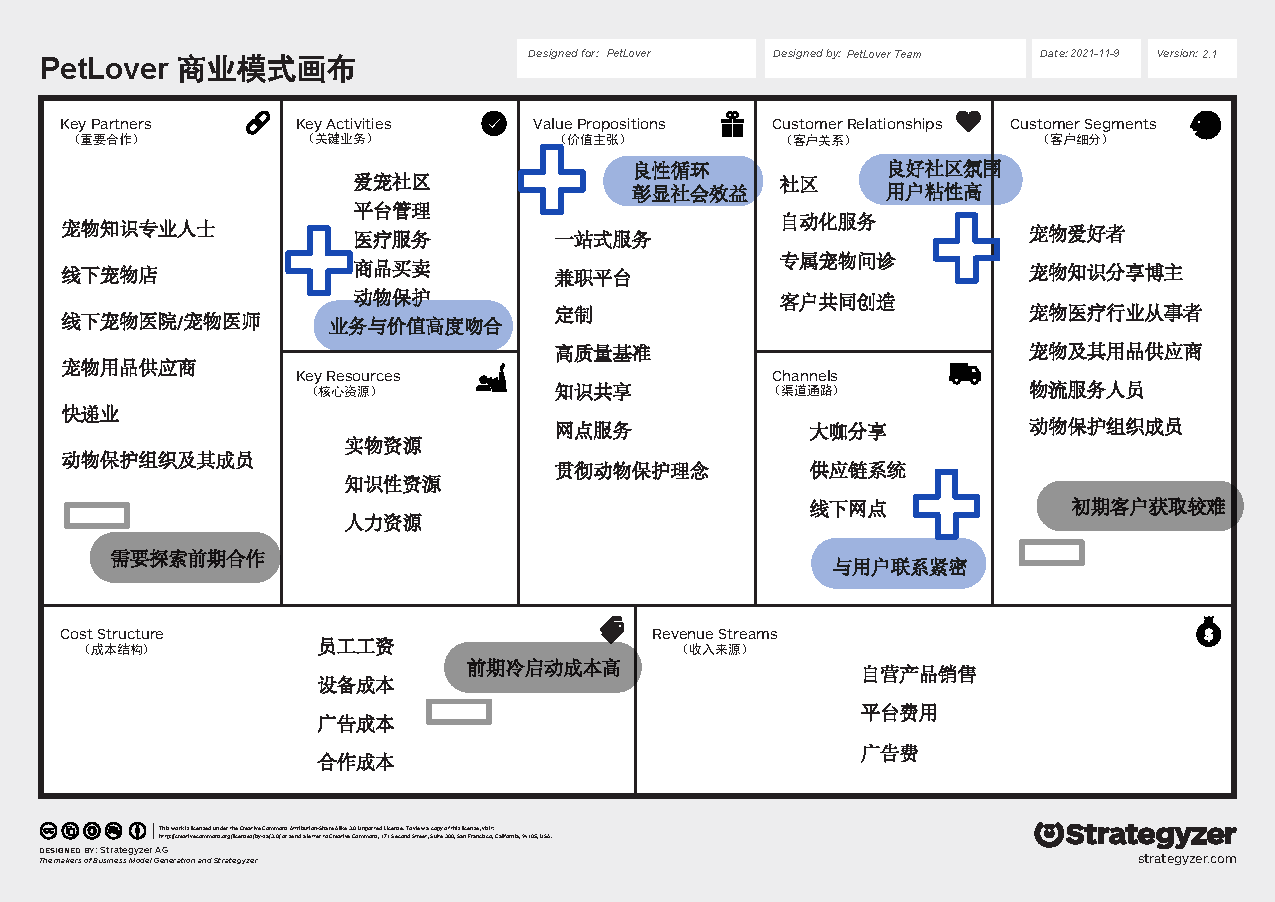
\includegraphics[scale=0.75]{总体评估.pdf}
\end{center}
加分项:\\
\begin{itemize}
  \item \textbf{价值主张}:良性循环
  \item \textbf{渠道通路}:与用户联系紧密
  \item \textbf{客户关系}:良好社区氛围
  \item \textbf{客户关系}:用户粘性高
  \item \textbf{关键业务}:业务与价值高度吻合
  \item \textbf{价值主张}:彰显社会效益
\end{itemize}
减分项:\\
\begin{itemize}
  \item \textbf{成本结构}:前期冷启动成本高
  \item \textbf{重要合作}:需要探索前期合作
  \item \textbf{客户细分}:初期客户获取较难
\end{itemize}

PetLover平台最突出的地方在于其价值主张、渠道通路以及客户关系上。一方面,在大咖分享的渠道通路以及客户关系的驱动下,平台容易形成用户共同创造的社区氛围,这会在用户群体中形成良性循环,用优质内容吸引用户、链接社群,再用社群绑定用户。另一方面,一站式服务的价值主张和线下网点的渠道通路让用户的时间成本得以降低,让用户从最初的围观者变为关注者,再从关注者升级为参与者,最后从参与者升级为消费者。这成为平台绑定用户的秘诀,也成为了平台吸引来优质合作者的手段之一。正是由于这些理由,PetLover的关键业务得以成为其价值主张的完美彰显,没有分毫冗余业务,大大提高了用户体验。

在社会效益与社会责任方面,PetLover平台以贯彻动物保护理念的价值主张、与中国小动物保护协会的重要合作形成标榜作用,在提高平台的社会影响力的同时还能吸引更多客户,让平台在更多渠道上得以推广,同时也发挥了平台自有的流量的价值。因此,无论是内容创作还是产品营销,都要坚持社会效益与社会责任不动摇。

PetLover平台总体上还是一个以社群为主的平台,因此我们对重要合作和客户细分的依赖较高。对于平台初期来说,我们面临一定的冷启动风险,即如何才能吸引来大量的用户、如何维持较高的日活量。因为往往一个优秀的宠物博主在其他平台已经积累了大量的笔记分享,在别的平台已经建立起了一整套完整的用户信息和用户生态,对于这类资深用户来说,切换平台的难度较大。因此我们平台在这一块必须要有能够吸引来博主的优势,例如从平台建立初期支付合作成本的角度考虑。对于初期阶段来说,我们也许无法在规模上取得优势,因此要尽可能在内容上取得优势,这也是我们的价值主张所欠缺的。 

放眼未来,PetLover平台需要以双管齐下的策略继续发展。一方面,平台需要坚持它在价值主张、渠道通路以及客户关系上的优势,继续营造由大咖分享带动的用户共同创造的社区氛围,推动自带线下网点的一站式服务,打造优质社群,发挥显著的增长潜力。另一方面,平台需要持续聚焦用户满意度,打造金牌内容质量,开拓新领域的业务合作,让平台能够吸引大量用户、维持较高日活,从而为优质社群的建立打下坚实的基础。

\subsection{SW 评估——从内部评估公司的优劣势}
\FloatBarrier
\subsubsection{价值主张评估}
\begin{table}[h]
  \centering
\begin{tabular}{|p{3.5cm}|c|p{10cm}|}
  \hline
  我们的价值主张与客户需求一致 & 5 & 我们提出的一站式服务的价值主张满足了养宠主人对宠物服务相关的需求;兼职平台则满足了宠物(用品)店主、宠物医师的兼职需求;高质量基准主张为用户提供了优质可靠的产品和服务;知识共享主张针对于亟需宠物饲养经验和相关知识的用户;网点服务主张为各地区用户提供线下网点的渠道;定制主张为饲养不同宠物、需求不同的用户提供针对性服务;贯彻动物保护理念则为动物保护志愿者提供了宣传平台。\\
  \hline
  我们的价值主张有很强烈的网络效应  & 4 & 我们平台的价值与平台用户的数量呈正相关性,尤其是对于兼职平台和定制社区的主张。对于兼职平台来说,使用平台的用户越多,兼职者获得的收入就越多,形成良性的正循环;对于定制社区来说,这是我们很重要的价值主张,定制社区是客户共同创造的良好环境,用户越多,产出的知识资源就越多,就会有更多人加入平台。\\
  \hline
  在我们的产品和服务之间有很强的协同效应 & 4 & 我们提供的产品都是紧紧依赖于我们所拥有的服务。例如爱宠商品买卖、爱宠社区等关键产品都需要以我们的一站式服务为前提;我们提供的医疗服务、平台管理则对应于我们为用户提供宠物购入后续的一系列便利产品——专属宠物问诊、宠物用品买卖等;我们的动物保护服务则提供宠物领养等相关产品。\\
  \hline
  我们的客户非常满意 & 4 & 我们平台提供的业务十分符合用户需求,真正实现了宠物一站式服务,切实地避免宠物主在各个平台间反复横跳,且服务水平良好,能够获得用户的好评;对于个别客户的不良反馈,我们也会及时反思并进行调整。\\
  \hline
\end{tabular}
\end{table}
\FloatBarrier
\subsubsection{成本/收入评估}
\begin{table}[h]
  \centering
\begin{tabular}{|p{3.5cm}|c|p{10cm}|}
  \hline
  我们受益于强劲的利润率 & 3 & 我们通过销售自营产品、收取线下宠物店、宠物医院平台费用、广告费来获得利润,由于多样化的成本结构,在计算实际利润时要对各种因素进行考虑。\\
  \hline
  我们的收益可以预测 & 3 & 我们的收入来源结构相对固定。但用户使用平台的频率难以预测,可能会在商品销售上的收入有所波动。此外,合作伙伴、广告商也不是一成不变的,平台费用和广告费也会产生变化。\\
  \hline
\end{tabular}
\end{table}
\begin{table}[h]
  \centering
\begin{tabular}{|p{3.5cm}|c|p{10cm}|}
  \hline
  我们有很多经常性收入和回头客 & 5 & 我们平台特有的宠物一站式服务和爱宠社区的业务可以留住顾客,尤其是刚刚从平台购入宠物的宠物主,后续需要在平台上进行一系列的诸如宠物用品购买、宠物疾病咨询、宠物饲养交流等活动;再加上平台对用户的自动化服务可以提醒用户所需,让用户继续在平台上消费,让平台有经常性的收入和稳定的回头客。\\
  \hline
  我们的收益来源是多样化的 & 4 & 我们的主要收入来源包括自营产品销售、平台费用和广告费,其中平台费用包括线下宠物店和宠物医院的入驻费用、宠物店销售商品的平台抽成、宠物问诊的平台服务费等。\\
  \hline
  我们的收益来源是可持续的 & 4 & 我们平台特有的宠物一站式服务和爱宠社区的业务可以保证平台有稳定的回头客,他们后续会在平台上进行一系列的诸如宠物用品购买、宠物疾病咨询、宠物饲养交流等活动,并且会将平台介绍给身边同样养宠的朋友们,让他们加入平台,形成持续稳定的收入来源。\\
  \hline
  我们在支出成本之前就有收入进账 & -5 & 我们的平台服务尚未搭建完成时,需要进行花费成本购入相关设备、推广平台品牌等工作,还不会有相关的收入来源。待平台搭建稳定后,才会吸引源源不断的用户和合作伙伴前来加入并产生平台收入。\\
  \hline
  我们提供客户真正想买的 & 5 & 我们深入分析并了解各类用户的诉求,站在他们的角度切实思考他们需要什么、平台应该提供什么。如平台重点宣传的一站式服务,就是要解决养宠新人对养宠知识不熟悉、对购宠渠道不了解的痛点,让他们放心地在平台上进行购买宠物以及后续一系列活动;再比如我们完善的供应链系统,将线下网点和用户家紧密链接,为用户提供了极大的便利,缩减了用户的成本。\\
  \hline
  客户完全接受我们的定价机制 & 3 & 除部分自营宠物用品等之外,其余产品诸如宠物、宠物用品、医疗服务费等均由相关卖家决定,平台可能会定期推出促销活动,但其余大部分时间客户能否接受定价取决于商家的定价。考虑到为了让平台运转良好,平台会对各个商家的定价进行规范,确保用户可以接受商品定价。\\
  \hline
  我们的成本可以预测 & 4 & 我们的成本结构较为固定,有员工工资、设备成本(服务器等)、广告成本(前期宣传平台)、合作成本(大咖引进、知识分享等)。除广告成本和合作成本稍有波动外,其余成本均可预测。\\
  \hline
  我们的成本结构和商业模式完全匹配 & 4 & 我们花费一定成本购买云服务器,聘请宠物医师、进行平台推广、邀请大咖进行经验分享,其目的都是为了最终建立一个健康、权威、友善的宠物服务及宠物交流平台,将不同宠物主通过平台联系在一起,并与各类重要合作伙伴展开合作,为用户提供更有价值的服务,这与我们的多边平台商业模式是匹配的。\\
  \hline
  我们的运营成本低且效率高 & 3 & 为了保证平台运营的高效率,我们需要定期维护平台和服务器,定期巩固与合作伙伴尤其是线下宠物店和宠物医院以及运输行业的良好合作关系,此过程所需的成本预计并不会低,但我们努力希望达到平台的高效率运营。\\
  \hline
  我们受益于规模效益 & 5 & 当平台的规模不断扩大,即意味着我们与更多重要合作伙伴展开合作(宠物店、快递业、宠物医疗、动物保护组织),并意味着我们需要增加更多的服务器和员工,但与此同时,平台就能够承载更多的客户,而平台本身作为一个为宠物店主和宠物医师等提供兼职的平台,将会创造更多的价值。\\
  \hline
\end{tabular}
\end{table}

\FloatBarrier
\subsubsection{基础设施评估}
\begin{table}[h]
  \centering
\begin{tabular}{|p{3.5cm}|c|p{10cm}|}
  \hline
  竞争对手很难复制我们的核心资源 & 4 & 我们的核心资源主要包括实物资源、知识性资源和人力资源。其中实物资源包括线下宠物店、宠物医院及服务器等设备,与我们达成合作的宠物店和宠物医院具有平台依赖性;知识性资源包括用户共同创造的宠物饲养指南、宠物医疗科普常识等社区知识资产,是使用平台的用户共同的资源,也是平台爱宠社区的特色资源,是竞争对手很难复制的。\\
  \hline
  我们的资源需求是可以预测的 & 5 & 我们可以根据平台的用户数量、用户在使用平台中的反馈(如平台使用流畅度、对宠物用品的具体需求、对宠物服务的具体需求等)、兼职人员的反馈(如兼职宠物医师反映咨询人数过多,则需要招募更多宠物医师)等方式进行资源需求预测,并根据实际情况采取相应的行动。\\
  \hline
  我们在恰当时间合理地调配核心资源 & 4 & 养宠作为现代人的一种精神需求,其实早在多年前就开始流行起来了。经过市场调研我们发现市面上已经存在数款宠物相关软件,但这些软件都只是单一聚焦于宠物购买、宠物用品售卖、宠物社区等模块,市面上目前没有一个能够提供一站式服务的宠物平台。此外,最近几年养宠物越来越盛行,我们正处在一个正确的时间进行核心资源调配,直面客户群体的迫切需求。\\
  \hline
  我们高效执行了关键业务 & 5 & 我们平台提供的服务与关键业务之间有着很强的协同效应,既然我们重点主张一站式宠物服务,我们就需要切实高效执行关键业务,将一站式服务深入贯彻。最近,我们新推出的“上门服务”也聚焦于高效率,将宠物用品送货到家,对于大型宠物用品(如猫爬架等)还提供组装服务,让用户感受到我们的专注。\\
  \hline
  我们的关键业务很难被复制 & 2 & 虽然我们的一站式服务在竞品平台上很少见,比较难以复制,但我们的爱宠社区、商品买卖等业务在其他宠物平台上均有普及,容易被复制。但总地来看,像我们平台这样提供一站式、多关键业务的形式,是其他平台难以做到的。\\
  \hline
\end{tabular}
\end{table}
\begin{table}[h]
  \centering
\begin{tabular}{|p{3.5cm}|c|p{10cm}|}
  \hline
  我们的执行质量很高 & 5 & 为了保证良好的客户体验,对于业务的执行,我们必须以高质量为标准:我们尽力维护爱宠社区的健康良好运行;对于商品买卖,我们始终进行规范和监督,保证提供客户需要的、并让客户接受我们的定价机制;对于医疗服务,我们坚持招募专业医师,与正规宠物医院进行合作;对于动物保护,我们始终不忘初心,让动物保护理念深入到每一个宠物爱好者乃至其他人群的心中。\\
  \hline
  我们很好平衡了内部业务和外包业务 & 4 & 我们的关键业务彼此相系,一系列业务都是在宠物饲养中不可或缺的,对于平台内部的业务,我们要认真对待,对于外部业务(如运输与快递业合作,宣传动物保护理念与动物保护组织进行合作)我们亦达到很好的平衡,保证平台运营良好,高效、高质量地执行关键业务,体现价值主张。\\
  \hline
  我们很聚焦,必要时与伙伴合作 & 5 & 我们聚焦于宠物相关的一系列服务,每一项服务和关键业务都离不开与重要合作伙伴的密切合作,从商品的供应、运输到售后,每一环都非常有必要与伙伴合作。\\
  \hline
  我们和重要合作伙伴的关系很融洽 & 5 & 线下宠物店、宠物医院、宠物用品供应商、快递业、动物保护组织等是我们关键业务得以开展的重要支撑,我们必须维持良好的合作关系。\\
  \hline
\end{tabular}
\end{table}
\FloatBarrier
\subsubsection{客户界面评估}
\begin{table}[h]
  \centering
\begin{tabular}{|p{3.5cm}|c|p{10cm}|}
  \hline
  我们的客户流失率低 & 5 & 我们既然提供了一站式服务,就希望用户对平台依赖性较强,从购买宠物到后续一系列宠物养护的需求再到爱宠社区交流养宠心得都可以在我们的平台上的以满足,并且我们高效率、高质量的服务也增加了用户对平台的信任,因此用户并不会轻易流失。\\
  \hline
  我们对客户群体的细分很详细 & 5 & 我们的客户群体细分为:宠物爱好者、宠物知识分享博主、宠物医疗行业从事者、宠物及用品供应商、物流服务人员、动物保护组织成员等,不同的客户群体对应于平台不同的关键业务和客户关系。\\
  \hline
  我们在持续不断地赢得新的客户 & 4 & 我们平台稳定的回头客会将平台介绍给身边同样养宠的朋友们,让他们加入平台,形成持续稳定的客户来源;随着平台品牌和影响力的不断扩大,也会吸引更多宠物店、宠物医院、快递行业公司、动物保护组织等加入平台建设,持续不断地赢得新客户。\\
  \hline
\end{tabular}
\end{table}
\begin{table}[h]
  \centering
\begin{tabular}{|p{3.5cm}|c|p{10cm}|}
  \hline
  我们的渠道通路运作效率高 & 4 & 我们通过大咖分享定期助力平台推广和活跃社区;通过逐步扩大的线下网络及其中的线下网点为各个地区的用户提供可靠的购买渠道;通过完善的供应链系统保障商品买卖及后续的运输、售后服务。\\
  \hline
  我们的渠道通路设置十分合理 & 4 & 我们的各个渠道通路各自发挥着其作用,如平台推广和活跃社区,提供可靠的购买渠道,保障商品买卖及后续的运输、售后服务等。\\
  \hline
  我们的渠道通路链接客户的能力强 & 3 & 我们的渠道通路中,大咖分享可以链接潜在的客户;供应链系统、线下网点渠道则可以将平台的长期用户很好地链接起来。但仍需要进一步加强渠道通路链接客户的能力,如何进行长期用户管理、加强用户忠诚度是我们需要持续考虑的问题。\\
  \hline
  客户能够轻易地看到我们的渠道通路 & 4 & 大咖分享是以宣传帖子、海报等方式进行宣传的,目的就是为了让客户看到;而供应链系统和线下网点则是客户实际生活中几乎每天都要接触到的渠道。\\
  \hline
  我们的渠道通路整合地很好 & 3 & 大咖分享能够宣传平台、活跃社区;线下网点渠道则可以提供实物资源,是进行商品买卖的可靠渠道;供应链系统保证了商品的供应、运输和售后。\\
  \hline
  我们的渠道通路创造出了范围效应 & 4 & 在扩展渠道通路的同时(如邀请更多大咖进行分享,扩展供应链系统、与更多快递公司进行合作,与更多线下宠物店、宠物医院展开合作使其成为线下网点等),可以吸引更多潜在客户加入平台,将宠物服务扩展至更多地区,让更多用户受益于平台的良好服务和便利性,从而收益更多。\\
  \hline
  我们的渠道通路完全匹配客户细分群体 & 3 & 我们的渠道通路中,供应链系统匹配于宠物及用品供应商和物流服务人员,线下网点匹配于宠物及用品供应商。但动物保护志愿者和广告商没有相对应的渠道通路。\\
  \hline
  我们的客户关系良好 & 5 & 我们的客户之间联系紧密。如爱宠社区维护了用户之间的关系,在用户共同创造知识性资源后关系会更加紧密;宠物爱好者依赖于宠物及用品供应商和物流服务人员进行商品供应运输;动物保护志愿者会在社区中和其他宠物爱好者分享动物保护的理念,形成正能量社区。\\
  \hline
  客户关系的品质与客户细分群体相匹配 & 4 & 	以平台非常重要的业务——爱宠社区为例,它为宠物爱好者用户们建立了社区的客户关系,诸多宠物爱好者齐聚社区,共同维持社区的健康和活跃,他们在社区中分享知识、交流心得、共同创造知识、创造价值,爱宠社区的品质就直接与客户群体匹配,决定了用户和平台的关系质量。\\
  \hline
  客户切换成本高,客户和我们紧密绑定 & 5 & 我们反复强调的一站式服务价值主张,就是为了解决宠物爱好者在其他多个平台之间反复横跳的痛点。我们平台的服务既减少了用户成本,又提供了优质的服务,爱宠社区也增加了用户粘性,用户没有理由轻易放弃体验良好的平台和自己在平台上创造的价值而切换到其他平台。\\
  \hline
  我们的品牌很强 & - & 尚无法评分,但如果我们能矢志不渝、不忘初心,坚持我们的高品质服务,持续推进平台高质量运营和建设,相信我们一定能打造更强的品牌,拥有一群忠诚度很高的客户群体,让平台越走越远。\\
  \hline
\end{tabular}
\end{table}

\FloatBarrier
\subsection{机会评估}
\subsubsection{价值主张中的机会}
\begin{table}[h]
  \centering
\begin{tabular}{|p{3.5cm}|c|p{10cm}|}
  \hline
  能通过把产品转换为服务而产生重复性收入吗? & 5 & 可平台把宠物医疗问诊和宠物用品买卖融入了宠物售卖中,一次性的宠物买卖可以变为后续养护宠物的服务型宠物消费,将收入可持续化以及重复化。\\
  \hline
  我们能更优地整合我们的产品或服务吗? & 5 & 平台主张一站式服务会利用各个模块的优势,整合服务来提供更好地宠物相关内容。同时线下店铺线上宣传模式有助于整合线下资源来为我们的客户提供更透明更多样的线下服务。\\
  \hline
  我们还能满足客户的哪些额外需求? & 1 & 由于平台一站式服务已经包含了大部分的宠物软件的服务业务,如果继续扩大业务需要考虑成本的扩增,目前平台不会考虑拓展业务来满足客户的额外需求。\\
  \hline
  我们的价值主张还可能做哪些补充和外延? & 4 & 在一站式服务的宠物社区方面,我们需要注重流量的引入,我们的宠物社区不仅仅要注重宠物饲养知识的分享,需要营造爆款,注重宠物自媒体,以更加娱乐的方式来打造社区,吸引更多的非宠物爱好者成为一个宠物爱好者来扩大流量。\\
  \hline
  我们还能为客户做哪些工作? & 1 & 目前平台无法继续整合更多的服务,比如自己进军具体的宠物制造业以及宠物医疗行业,因此我们还能为客户做的工作有限。\\
  \hline
\end{tabular}
\end{table}

\FloatBarrier
\subsubsection{成本/收入的机会}
\begin{table}[h]
  \centering
\begin{tabular}{|p{3.5cm}|c|p{10cm}|}
  \hline
  (R\$)我们能将一次性交易收入改为重复性收入吗? & 3 & 在自营产品销售方面,我们可以使用月卡、年费卡等制度来给客户提供一定的优惠来吸引客户购买,将一次性的商品买卖的收入转化成月卡、年费卡的重复持续收入。同时平台费用,广告费用本身不是一次性交易收入,是可以重复持续得到收益的。\\
  \hline
  (R\$)客户还愿意为哪些元素买单? & 1 & 平台一站式服务基本涵盖了宠物服务的多个方面,客户没有还希望买单的元素。\\
  \hline
  (R\$)我们有内部交叉销售或者和合作伙伴交叉销售的机会吗? & 5 & 平台一站式服务内部就存在很多的交叉销售的,宠物买卖之后推销宠物用品销售以及宠物在线问诊服务。同时我们将流量引导向我们线下合作的宠物店和宠物医院来为合作伙伴提供交叉销售的机会,让宠物后续的护养推向合作伙伴。\\
  \hline
  (R\$)我们还能增加或者创造哪些其他的收益来源? & 3 & 我们后续存在将宠物问诊专业化、规模化的可能,因此我们可以从中收取高质量的宠物问诊的中间收取平台运营的中间费用。\\
  \hline
\end{tabular}
\end{table}
\begin{table}[h]
  \centering
\begin{tabular}{|p{3.5cm}|c|p{10cm}|}
  \hline
  (R\$)我们能提价吗? & 3 & 当平台流量做大了只有,我们的平台费用提升并不会引起客户的反感,因为加入平台宣传能够为他们带来足够大的利益收入。同时广告费也同理。由于宠物商品买卖价格透明,我们不太存在提价的可能。\\
  \hline
  (C\$)我们能在哪里削减成本? & 1 & 由于平台运行、推广、合作的成本都是硬性的支出,因此平台不太可能存在削减成本的可能。\\
  \hline
\end{tabular}
\end{table}

\FloatBarrier
\subsubsection{基础设施中的机会}

\begin{table}[h]
  \centering
\begin{tabular}{|p{3.5cm}|c|p{10cm}|}
  \hline
  (KR)我们能用更低廉的资源获得同样的效果吗 & 1 & 为了平台平稳运行需要,实物资源以及人力资源是必要的,如果用更加低廉的资源会威胁平台的运行稳定。同时宠物社区里面的专业知识性是平台流量的入口,需要大量投入优质资源,否则社区的质量会受到严重威胁,导致平台市场份额削减。\\
  \hline
  (KR)哪些核心资源合适转移给合作伙伴 & 1 & 我们平台的运行需要自己把握,无法转移给合作伙伴。知识性资源是平台的核心,需要平台来把控,无法转移外包。\\
  \hline
  (KR)哪些核心资源开发不足 & 1 & 实物资源以及人力资源用于平台运行,知识资源充分支撑了宠物社区。\\
  \hline
  (KR)我们有没有哪些没有使用的知识资产是对别人有价值的 & 1 & 我们暂时不存在没有使用的知识资产是对别人有价值。我们的知识资产主要是在平台管理以及宠物社区方面,但是这是我们的核心,需要为平台服务。\\
  \hline
  (KA)我们能将某些关键业务标准化吗 & 4 & 平台管理方面,社区内容的审核流程可以标准化。医疗服务,上门服务方面可以通过规范来提供更加标准化的服务。而动物保护,商品买卖本身就是等多样的服务本身\\
  \hline
  (KA)我们能提升整体效率吗 & 5 & 平台一站式服务目的就是为了整合宠物相关方面的各个服务来减少客户在不同平台之间的切换成本。平台整合相关服务,目标会更加专注,因此整体效率提升的可能性更高。\\
  \hline
\end{tabular}
\end{table}
\begin{table}[h]
  \centering
\begin{tabular}{|p{3.5cm}|c|p{10cm}|}
  \hline
  (KA)IT能够提升效率吗 & 1 & 平台本身就是一个社交购物软件平台,IT技术是自身具备的,平台的目标之一就是利用IT来整合线下资源来提升客户的效率,所以在没有新技术更迭的情况下能提供的效率提升是有限。\\
  \hline
  (KP)有外包的机会吗 & 4 & 宠物医疗是外包给我们合作的线下宠物医院的,上门服务可以交付给宠物店,动物保护是由CSAPA志愿者组织开展的。平台管理是核心无法外包。\\
  \hline
  (KP)与合作伙伴扩大合作能够帮助我们聚焦核心业务吗 & 1 & 我们基本已经将可以外包的核心活动外包给了合作伙伴,平台聚焦商品买卖,平台管理以及宠物社区这些平台的核心业务。\\
  \hline
  (KP)有与合作伙伴交叉销售的机会吗 & 5 & 平台将流量引导向我们线下合作的宠物店和宠物医院来为合作伙伴提供交叉销售的机会,让宠物后续的护养的服务推向合作伙伴。\\
  \hline
  (KP)合作伙伴的渠道能够帮我们更好地连接客户吗 & 5 & 线下的宠物店和宠物医院的线下网点,帮助我们避免部署线下店铺连接客户。同时,快递业合作伙伴的物流系统帮助扩增我们的供应链系统,让我们的宠物、宠物商品更安全快捷地抵达客户的手中。同时宠物医院的线下网点的专业宠物医生也帮助我们维系宠物问诊的客户关系。\\
  \hline
  (KP)合作伙伴能够补充我们的价值主张吗 & 1 & 合作伙伴不能够补充我们的价值主张。平台本身是基于自身独特的价值主张来寻找我们的合作伙伴的,因此补充价值主张比较困难。\\
  \hline
\end{tabular}
\end{table}

\FloatBarrier
\subsubsection{客户界面的机会}
\begin{table}[h]
  \centering
\begin{tabular}{|p{3.5cm}|c|p{10cm}|}
  \hline
  (CS)我们如何从一个增长的市场中获益? & 5 & 我们要做好宠物社区的流量入口,把握增长市场中更多的客户,提升用户粘性,在宠物购买服务的后续收益中获取利益。\\
  \hline
  (CS)我们能服务新的用户吗? & 3 & 在宠物买卖方面,除了宠物店,可以面向宠物活体培育企业或组织等新用户,为他们提供宠物买卖的展示窗口,他们不必自身打造对外展示平台,专注于高质量的宠物活体培育活动。\\
  \hline
  (CS)我们能够通过更细致地给客户分类来提供更好地服务吗? & 5 & 一些宠物爱好者由于各种原因本身可能不会饲养宠物,但是他们会观看一些宠物视频来获得内心的慰藉。宠物社区应该关注这一类客户细分,因此宠物爱好者可以进一步细分。\\
  \hline
  (CH)我们如何能提升渠道的效率和效益? & 3 & 大咖分享要有用户针对性,选取最具代表性来提高平台的标识度。供应链系统可能需要外包给专业的快递物流企业来整合物流优势。同时专属服务要根据用户画像来推荐,提高用户使服务的几率来提升渠道的效率和效益。\\
  \hline
\end{tabular}
\end{table}
\begin{table}[h]
  \centering
\begin{tabular}{|p{3.5cm}|c|p{10cm}|}
  \hline
  (CH)我们能更好地整合渠道吗? & 3 & 线下网点和我们的供应链系统可以融合,让线下网点成为物流的暂存点。例如,大型宠物用品可以由线下宠物店提供安装服务,宠物医院可以直接让医疗用品作用于宠物上。\\
  \hline
  (CH)我们能够找到补充性的新渠道伙伴吗? & 1 & 不太可能在合作伙伴找到我们的渠道具有互补性的渠道通路。设计之初就已经很好的考虑到了合作伙伴可以给我们提供的渠道,再找到新的具有互补性的渠道通路困难。\\
  \hline
  (CH)我们能够通过直接服务客户来提升利润吗? & 1 & 如果平台亲自部署供应链系统和线下网点会带来成本的极大提升,可能会导致成本无法控制,资产模式过重,从而使利润下降。\\
  \hline
  (CH)我们能更好地匹配渠道和客户群体吗? & 2 & 我们的渠道已经较好地匹配了客户群体。例如在线下网点匹配了宠物爱好者以及宠物医疗从业者,供应链系统匹配了宠物用品商以及快递从业人员。\\
  \hline
  (CR)有可能提升客户的跟进效果吗? & 4 & 平台可以通过线上线下结合的方式对用户进行跟进,通过线上的产品购买,问诊服务以及线下网点线上预约等模块进行直接的服务意见反馈。同时,我们的宠物社区中审核人员会对用户发言进行及时的审核反馈,并且宠物社区存在直接用户反馈功能。最后我们可以及时和线下网点进行跟进,询问提供服务过程中的困难。\\
  \hline
  (CR)如何能让我们与客户的关系更加紧密? & 5 & 通过将宠物社区与用户共同创造增加客户粘性,提供高质量的宠物用品以及可保证的宠物问诊来进一步提高我们与宠物爱好者之间的密切关系。为宠物医疗从业者提供兼职的宠物问诊来提高他们的职业成就感来让关系更加密切。\\
  \hline
  (CR)(CR)我们能够在定制化上面做改进吗? & 2 & 平台价值主张就存在定制化,我们在社区以及自动化服务(提供模块导航)的客户关系上已经做了很高的定制化。社区内容可以根据用户画像进行推荐,同时自动化服务会智能推荐用户希望的服务。我们可以在专属宠物问诊方面根据宠物种类进一步做一些定制化的细分。\\
  \hline
  (CR)我们如何能够提升客户的切换成本? & 1 & 平台提供的一站式服务已经能够极大的减少了客户在宠物服务方面的各个需求,不需要在不同平台之间,因此通过一站式服务,我们已经增加了用户的切换成本。\\
  \hline
  (CR)我们识别并“炒掉”了没有利润的客户了吗?如果没有,为什么? & 3 & 在客户中动物保护志愿者以及部分宠物爱好者(没有对平台产生直接利润)我们并没有“炒掉”。由于动物保护是我们价值主张中的一部分,需要动物保护志愿者成为我们的客户来贯彻价值主张,提高平台的声誉。同时部分宠物爱好者有潜力为平台产生利润,例如被平台内容吸引从而购买宠物等。\\
  \hline
  (CR)我们需要让某些客户关系变得可以自动维护吗? & 3 & 我们可以自动维护宠物爱好者以及宠物医疗从业者的关系。平台可以设计自动化的内容,为宠物爱好者推荐合适的产品与信息,为宠物医疗从业者提供咨询问题。但是我们需要自动跟进宠物用品商之间的关系。\\
  \hline
\end{tabular}
\end{table}

\FloatBarrier
\subsection{威胁评估}
\subsubsection{对价值主张的威胁}
\begin{table}[h]
  \centering
\begin{tabular}{|p{3.5cm}|c|p{10cm}|}
  \hline
  存在可替代的产品和服务吗? & 3 & 在一站式服务的价值主张中,我们在各个模块都存在替代的服务和产品。首先,专门的宠物用品电商平台波奇宠物、E宠会和我们主要竞争宠物用品销售。其次,宠物在线问诊服务方面,有人人宠,爱宠医生等专业的宠物医疗在线问诊平台与我们竞争。在宠物买卖方面,有宠物市场,得宠等专业宠物活体买卖的平台。在宠物社区方面并没有以此为核心业务的平台,这也是PetLover平台的核心优势,但是优质宠物内容存在当前大流量的视频社交平台如B站,抖音等的影响。线下店铺线上宣传模式,是PetLover的突出核心,能够整合零碎的线下宠物店,宠物医院等的实体资源,目前并没有类似的竞争队友。\\
  \hline
  竞争对手会报出更有竞争力的价格,或者提供更好的价值吗? & 1 & PetLover提供定制化的一站式服务,注重宠物社区,以及线下店铺线上宣传模式整合零碎的线下资源会提供独特的价值,并没有竞争对手来和我们竞争。同时PetLover由于可以整合不同资源的,利用该优势提供更有竞争力的商品价格以及服务价格。\\
  \hline
\end{tabular}
\end{table}

\FloatBarrier
\subsubsection{对成本/收入的威胁}
\begin{table}[h]
  \centering
\begin{tabular}{|p{3.5cm}|c|p{10cm}|}
  \hline
  (R\$)我们的利润受到竞争对手的威胁吗?是技术原因造成的吗? & 4 & 我们的利润受到竞争对手的威胁,是平台流量的原因。自营产品销售收入受到大型电商平台(如京东、淘宝、拼多多)的宠物细分模块的威胁。PetLover平台的流量、知名度与客户信任度不及大型电商平台,客户会选择在大型电商平台宠物用品细分模块购买产品。同时大型电商平台存在规模效应,与宠物用品生产工厂会存在直销等模式,单件商品成本会低廉。广告收入在PetLover平台流量少的情况下并不能成为占比高的收入。但是O2O的线下店铺线上推广的模式对线下宠物实体店有良好的宣传效果,平台费用持续增加。O2O模式下平台流量存在提升的空间,因此上述威胁存在减缓的可能。\\
  \hline
  (R\$)我们过多地依赖某一项或多项收益来源吗? & 4 & 广告费,自营产品销售以及平台费根本上都来自于流量带来的收益。PetLover平台存在过多地依赖流量带来的变现收入的收入结构。要做好流量PetLover平台就必须要把宠物社区和用户共同创造的流量入口把关好。\\
  \hline
  (R\$)未来有哪些收益来源会消失? & 1 & 未来PetLover平台做好宠物社区和用户共同创造的流量入口后,流量变现带来的广告费,自营产品销售以及平台费会增加。这些收益会一直伴随着平台的成长。\\
  \hline
  (C\$)哪几项成本会变得无法预测? & 2 & 随着平台体量变大,合作成本会变得无法预测。PetLover平台提供一站式服务,在宠物服务方面需要和线下宠物店以及宠物医院合作,支撑平台如上门服务等成本高的服务,同时在宠物用品销售方面,宠物线下用品店的上门取件业务的快递业合作成本也会增加。PetLover本质是一个购物社区软件,支撑一个软件平台运行的成本可以被软件领域专家预估得到的,因此其他成本(员工工资,设备成本)可以被预估。在平台体量增大期间,需要引入宠物自媒体的知名博主引流,广告成本会持续增加,但广告成本是可以被计划的,因此也可以被预估。\\
  \hline
  (C\$)哪些成本的增加会快过它们所支撑的收入?& 3 & 在合作成本中,一站式服务的上门服务首先需要与线下的宠物店和快递业合作,需要支出一定的合作成本之后,平台才会得到用户支付该高附加值服务的收益。如果盲目扩大该服务会存在成本的增加会快过它所支撑的收入的情况。\\
  \hline
\end{tabular}
\end{table}

\FloatBarrier
\subsubsection{对基础设施的威胁}
\begin{table}[h]
  \centering
\begin{tabular}{|p{3.5cm}|c|p{10cm}|}
  \hline
  (KR)我们会面临某些资源的供应短缺吗? & 2 & 随着互联网产业蓬勃发展,支撑PetLover软件运行的实体资源和人力资源供应短缺出现的可能性较低。但是支持宠物社区这个流量入口的知识性资源,例如可以制作优秀的宠物分享视频、宠物饲养教程的博主,会存在需要被知名视频社交软件,如B站、抖音、快手等争抢导致短缺的可能。\\
  \hline
  (KR)资源的质量能够保障吗? & 3 & 在平台日常运行方面,支撑PetLover软件运行的实体资源(服务器等)的质量是可以保障的。但是优秀的软件人才需要高薪水才能留住,人力资源质量方面存疑。知识性资源是由可以制作优秀的宠物分享视频的博主等优秀的内容创造者创造的,需要资金才可能留住高质量的内容创造者,得到高质量的知识性资源。\\
  \hline
  (KA)哪些关键业务会被打扰?& 1 & PetLover的关键业务在资金以及与合作伙伴合作稳定的前提下基本可以正常运行。但是上门服务存在宠物店上门服务人员有限的情况而被推迟打扰的情况。\\
  \hline
  (KA)我们的活动质量会受到威胁吗?& 3 & 宠物社区需要专门的风纪人员去把关内容管理平台,禁止负面内容产生来保证社区质量。医疗服务存在不专业人员进入以及从业人员专业知识不过关等现象,需要进行考核。上门服务的考验最大,可能存在上门人员技术不过关无法按质量完成的问题,需要特别注意。\\
  \hline
  (KP)我们有可能会失去哪些合作伙伴& 2 & PetLover平台围绕宠物为中心,给线下的宠物医院,宠物店提供了流量的入口,给他们带来巨大的声誉效益,他们是平台的最忠诚的合作伙伴。同时以动物保护理念为价值主张的宠物平台仍未出现,只要把关好动物保护活动的质量,不出现丑闻,CSAPA也是我们的忠诚的合作伙伴。宠物用品供应商和快递业需要我们主动和他们进行协商洽谈,否则会有丢失的风险。\\
  \hline
  (KP)我们的合作伙伴有可能和竞争对手合作吗?& 1 & 由于专门营造宠物社区的平台仍未出现,我们以宠物社区为流量的入口,做好宠物社区把握住流量不流向竞争对手,以社区为核心拓展到宠物问诊,宠物用品销售等,为我们的合作伙伴提供可持续的利益,我们就可以保证合作伙伴不会和竞争对手合作。\\
  \hline
  (KP)我们是不是过分依赖某些合作伙伴?& 1 & 平台作为宠物用品销售的下游,宠物用品商以及快递业希望能够与我们建相互建立关系。由于平台的核心是流量,我们只要做好了宠物社区这个流量的入口,我们的合作伙伴(宠物店、宠物医院)是流量的出路,合作伙伴会主动依赖我们,而不是我们过于依赖合作伙伴。\\
  \hline
\end{tabular}
\end{table}

\FloatBarrier
\subsubsection{客户界面上的威胁}
\begin{table}[h]
  \centering
\begin{tabular}{|p{3.5cm}|c|p{10cm}|}
  \hline
  (CS)我们的市场很快会饱和吗?& 1 & 在市场调研中,中国的宠物行业市场仍未规范,横向对比发达国家的宠物行业规模,宠物行业市场有着持续向上扩增的产业趋势。\\
  \hline
  (CS)有竞争对手在威胁我们的市场份额吗?& 3 & 中国宠物行业正在出现一些大资本,如新瑞鹏宠物医疗集团,正在进行行业内大量企业兼并与融合,试图成为宠物行业巨头。但是他们布局在实体产业,而PetLover以宠物社区为核心的竞争对手仍未壮大,我们的市场份额有巨大的产生空间。\\
  \hline
  (CS)客户转投竞争对手的可能性有多高?& 2 & 平台独特的线下线上模式会牢牢把握住线下宠物医院和宠物店。根据市场调研,目前以宠物社区与优质内容为流量入口的平台仍然为出现,但是存在由于社区内容质量下降导致流量流失的情况,流量流失的主要会在社交视频平台如B站、抖音等的优秀宠物自媒体,宠物爱好者的丢失会使得宠物医疗从业者存在转投其他平台的风险。\\
  \hline
  (CS)我们市场中的竞争多快会变得白热化?& 3 & 当前宠物软件平台仍呈现百花齐放的状况,每个平台都有自己专注的模块,把握住自己的客户细分。PetLover需要和他们在每个模块进行竞争来获得市场份额,竞争白热化即将到来。\\
  \hline
  (CH)竞争对手会威胁我们的渠道吗?& 2 & 供应链系统和快递业合作,竞争对手无法威胁。线下网点因为模式独特的原因,没有其他平台推广,在该方面目前仍然没有竞争对手。专属服务需要邀请专业人员(兽医)来维护渠道,如果竞争对手体量很大,会威胁到我们的渠道。在大咖分享方面,存在大流量平台的威胁。\\
  \hline
  (CH)我们的渠道有变得和客户不相关的危险吗?& 1 & 我们的渠道如大咖分享、专属服务、线下网点等都是面向我们的客户细分的,我们不太存在渠道有变得和客户不相关的危险。\\
  \hline
  (CR)我们的客户关系有可能恶化吗?& 1 & 由于平台管理是PetLover的核心业务,我们会注重平台用户共同创作的内容来维护社区。同时我们的专属宠物问诊确保咨询兽医的专业性。平台会提供自动化服务来引导客户使用平台,我们的客户关系恶化可能性不大。\\
  \hline
\end{tabular}
\end{table}

\FloatBarrier
\section{蓝海战略}

蓝海战略是通过来价值创新来拓展非竞争性市场空间的战略,规避竞争,创造并获取新需求,打破价值与成本互替定律,追求差异化和低成本,把企业行为整合为一个体系。在这一部分PetLover团队选择价值主张方向进行对第二阶段的商业模式画布探究。

\subsection{为什么优先选择价值主张方向进行探究?}

商业模式重要,价值定位先行。价值主张确认了公司对消费者的实用意义,对刚刚起步和进入瓶颈的企业,创新价值主张意味着生存与发展。我们认为成本影响方向强调的是在企业自身角度对投资与获取价值的衡量,对客户影响方向强调的是站在客户的角度衡量产品带给客户自身价值的衡量,而从价值主张方向进行探究能兼顾企业自身的需求和客户自身的需求,既能回答客户真正所关心的“我可以为你带来什么?”、“我可以超出你的什么期待”等问题,又能通过价值主张对企业成本、收益等进行探究。

\paragraph{依据:}《价值主张是商业模式的灵魂》(http://blog.sina.com.cn/s/blog\_508ef4740102x3wj.html)

吸引顾客的永远都不是产品和服务本身,而是为其所创造的价值感觉,你和其他同行业企业的差异化不在于你的产品本身,而是与他人不同的价值感受。平庸的企业只会制造产品;优秀的企业只会销售产品;卓越的企业才能创造价值。

\subsection{对价值主张方向的探究}
\begin{center}
  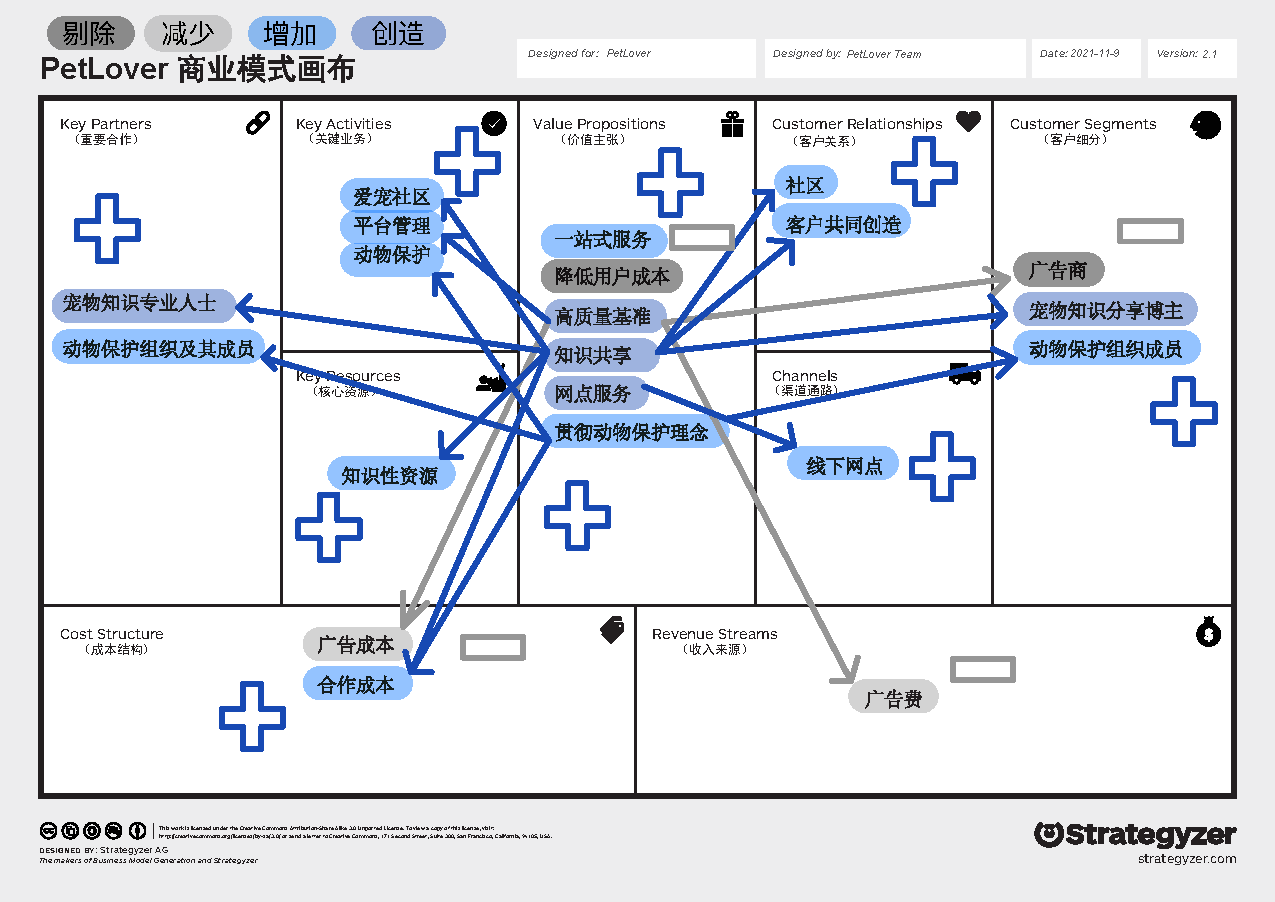
\includegraphics[scale=0.75]{价值主张.pdf}
\end{center}

\begin{itemize}
  \item \textbf{剔除}:缩减用户成本、广告商
  \item \textbf{减少}:广告费、广告成本
  \item \textbf{增加}:一站式服务、贯彻动物保护理念、社区、客户共同创造、线下网点、动物保护组织成员、合作成本、知识性资源、爱宠社区、平台管理、动物保护、动物保护组织及其成员
  \item \textbf{创造}:保证质量、网点服务、知识共享、宠物知识分享博主、与宠物知识专业人士的合作
\end{itemize}

对于\textbf{一站式服务},团队最终决定要对其投入增加。经过调研,目前市场上与我们类似的产品如E宠商城、爱宠大陆、宠物商城等应用大多服务单一,或只提供问答社区(爱宠大陆),或只提供宠物及其用品买卖(宠物商城)......宠物相关应用用户的一大痛点在于如何在克服跨平台寻求服务,他们希望得到方便快捷的宠物相关一站式服务(宠物社区论坛、宠物生活服务、宠物医疗服务、宠物商品买卖、宠物商品配送等),宠物一站式服务在当今宠物市场仍然属于蓝海。因此增加对一站式服务的价值主张的投入能够提高我们的核心竞争力。\textbf{该项结论的相关讨论可见商业模式环境→行业影响力和SW评估中的价值主张评估}

任何平台都需要有平台文化和人文关怀底蕴才能在后续发展中更有竞争力,团队对\textbf{贯彻动物保护理念}的价值主张进行增强,同时鼓励动物保护组织(如中国小动物保护协会)及其成员入驻平台论坛,即增强\textbf{与动物保护组织(如中国小动物保护组织)及其成员的合作},增强关键业务中的\textbf{动物保护}业务,在升华平台底蕴的同时还可以吸引更多的平台客流量,提高平台的社会影响力,为后续平台的推广打基础。\textbf{该项结论的相关讨论可见商业模式环境→市场影响力→市场分类→哪个细分市场在萎缩?哪个边缘细分市场值得关注?和商业模式环境→市场影响力→市场问题}

对于\textbf{缩减用户成本},我们需要从价值主张中剔除这个要点。因为所有宠物相关应用在为用户提供线上服务的时候都具有缩减用户成本(搜索成本、行动成本等)的作用,虽然不同应用有可能在缩减的效果上有所差别。它作为价值主张不仅没有给PetLover平台带来竞争力的提升,而且让平台商业模式画布略显冗余。\textbf{该项结论的相关讨论可见威胁评估中→对价值主张的威胁}

经过讨论,我们决定画布价值主张中创造“\textbf{高质量基准}”要点,PetLover平台的主营业务是宠物社区论坛和宠物及其商品买卖,因此社区论坛问答的内容质量和商品质量与性价比是用户考量的重要因素之一,只有高质量的问答内容和商品和才会为平台赢得更多的价值,确保用户都能习得养宠的正确“姿势”和购买物美价廉的宠物及其用品,增加用户体验。对于客户体验与产品质量的讨论可见依据1。依据1中还提到构成客户体验的关键组成部分是过程质量,用户使用PetLover平台的被服务体验非常重要,因此我们要将关键业务中的\textbf{平台管理}进行增强。另外,虽然商业模式环境板块中我们提到广告业在突飞猛进的发展,但经过社会调研,用户面对爆炸式的广告增长冲浪体验逐渐变差,参考依据2可知,我们需要对\textbf{收入来源中的广告费、成本结构中的广告成本}进行适当缩减。另外需要剔除客户细分中的广告商,因为提供广告的往往是宠物及其用品供应商和宠物服务机构等,存在重叠部分。\textbf{该项结论的相关讨论可见机会评估→客户界面的机会→所有打分点}

根据社区论坛具有问答的性质,我们在价值主张中创造了新的要点——\textbf{知识共享}。知识共享是当今共享时代的大趋势,PetLover面向的用户往往需要解决宠物相关的问题,大部分养宠人士所掌握的知识不足以支持他们为宠物提供贴心的照顾,因此PetLover平台会邀请和吸引宠物知识专业人士和大咖入驻平台,分享他们关于宠物如不同宠物种类品性、宠物疾病表现等相关知识,同时我们主张"知识无门槛",因此平台对知识分享不会收取相关费用,但允许博主将知识设置为付费或免费,同时会提供创作激励,相关调研见依据3。另外还在客户细分中创造了“\textbf{宠物知识分享博主}”要点,增加了\textbf{与宠物知识专业人士的合作},强调PetLover平台的问答服务,需要同时加强\textbf{社区和客户共同创造}两种客户关系,增强\textbf{爱宠社区}关键业务。另外我们修改了客户关系中的社区描述\textbf{该项结论的相关讨论可见商业模式环境→市场影响力→需求和诉求→客户需要什么?在客户需求中,哪些没有得到满足,最大的缝隙在哪里?}

我们商业模式画布中渠道通路有线下网点,但是价值主张中没有对应的要点,于是我们在价值主张中创造了\textbf{网点服务}要点,我们在各地加盟宠物服务网点,为辐射区域内的用户提供宠物的一系列服务,包括宠物生活服务、宠物医疗服务、商品配送服务等等,每个线下网点提供的服务范围可以有所不同。\textbf{该项结论的相关讨论可见商业模式环境→宏观经济影响→经济基础设施→你所处市场的(公共)基础设施有多优良?你如何评价交通、贸易、学校质量,以及连接供应商和客户的便利度?}

\subsection{依据}
\paragraph{1、《客户体验=产品质量+过程质量 》(https://www.sohu.com/a/316300940\_120120706)}该报告总结了一个要点:客户体验是一个企业的核心竞争力。而客户体验需要产品质量和服务过程质量的双重保证,这就需要在价值主张中融合保证质量要点。
\paragraph{2、《如何平衡产品广告变现与用户体验?》(http://www.woshipm.com/pmd/745206.html)}广告变现与用户体验的平衡,是在产品商业价值与用户价值之间进行抉择,找准两者之间的平衡点是产品可持续发展的关键。随着移动互联网的加速普及、“移动优先”消费趋势愈加深入,以及基于大数据的精准营销成为现实,移动广告自然就迎来了最美好的时代,广告变现过猛易会伤害用户体验,运营者要保持广告节制,合理而正确地规划广告位,追求原生广告和创意广告。
\paragraph{3、《知识的预期,互联网人在线教育的价值和洼地》(http://www.woshipm.com/it/553814.html)}在知识的变现下,也许不求所见即所得,但使更多的知识消费不仅是被包装,而是可被预期。知识共享的几种形式有社群分享、工具分享、标准化课程等。应该庆幸有越来越多的知识被分享和传播,也许解惑他人,也许彼此成长,让这个成长过程多一些亮光,少一些懵懂。在知识的变现下,也许不求所见即所得,但使更多的知识消费不仅是被包装,而是可被预期。
\section{画布更新}

\subsection{整体描述}

总体来说,我们增强了平台的核心价值主张,同时缩减无法突出平台核心竞争力和特色的主张。基于价值主张向左右两边的基础设施和客户界面进行调整,更改了成本与收入。

在价值主张方面,许多平台都会从用户的需求出发,缩减用户成本是一个好的平台的内在普遍共性,因此我们删除了缩减用户成本。一个优质的线上爱宠社区是平台一大特色,我们希望以高质量的宠物内容提升平台的知名度,以高质量的宠物在线问诊以及线下服务奠定发展基础,因此强调了高质量基准。同时我们希望我们的社区不是专家的,知名宠物自媒体的社区,每个在社区的爱宠人都能够为社区建设出力,说出自己的养宠心得体会,因此我们强调了知识共享。PetLover一直希望能够线上整合零碎的线下宠物店和宠物医院,无论城市的发达与否,宠物主都能够享受到高质量的宠物服务,因此把线下网点的渠道通路进一步提升为我们新的价值主张——网点服务,并强调了线上线下的一站式服务。同时贯彻动物保护理念是平台的生命力所在,进一步得到增强。

在客户界面上,根据上述的价值主张的调整,在客户关系方面,我们强调了社区以及客户共同创造,同时希望能够从在线社区拓展到线下宠物交友圈社区;在渠道通路方面,强调了线下网点的重要性;在客户细分方面,为了保证社区质量,减少了广告商,同时增加了宠物知识分享博主的客户细分,强调了动物保护组织成员。

在基础设施上,在关键业务中强调了爱宠社区构建,平台管理以及动物保护;在核心资源上强调了知识性资源;在重要合作中,增加了宠物知识专业人士,强调了动物保护组织及其成员。

在收入与成本上,为了高质量基准的服务,我们削减了广告成本

\subsection{更新后画布}
\begin{center}
  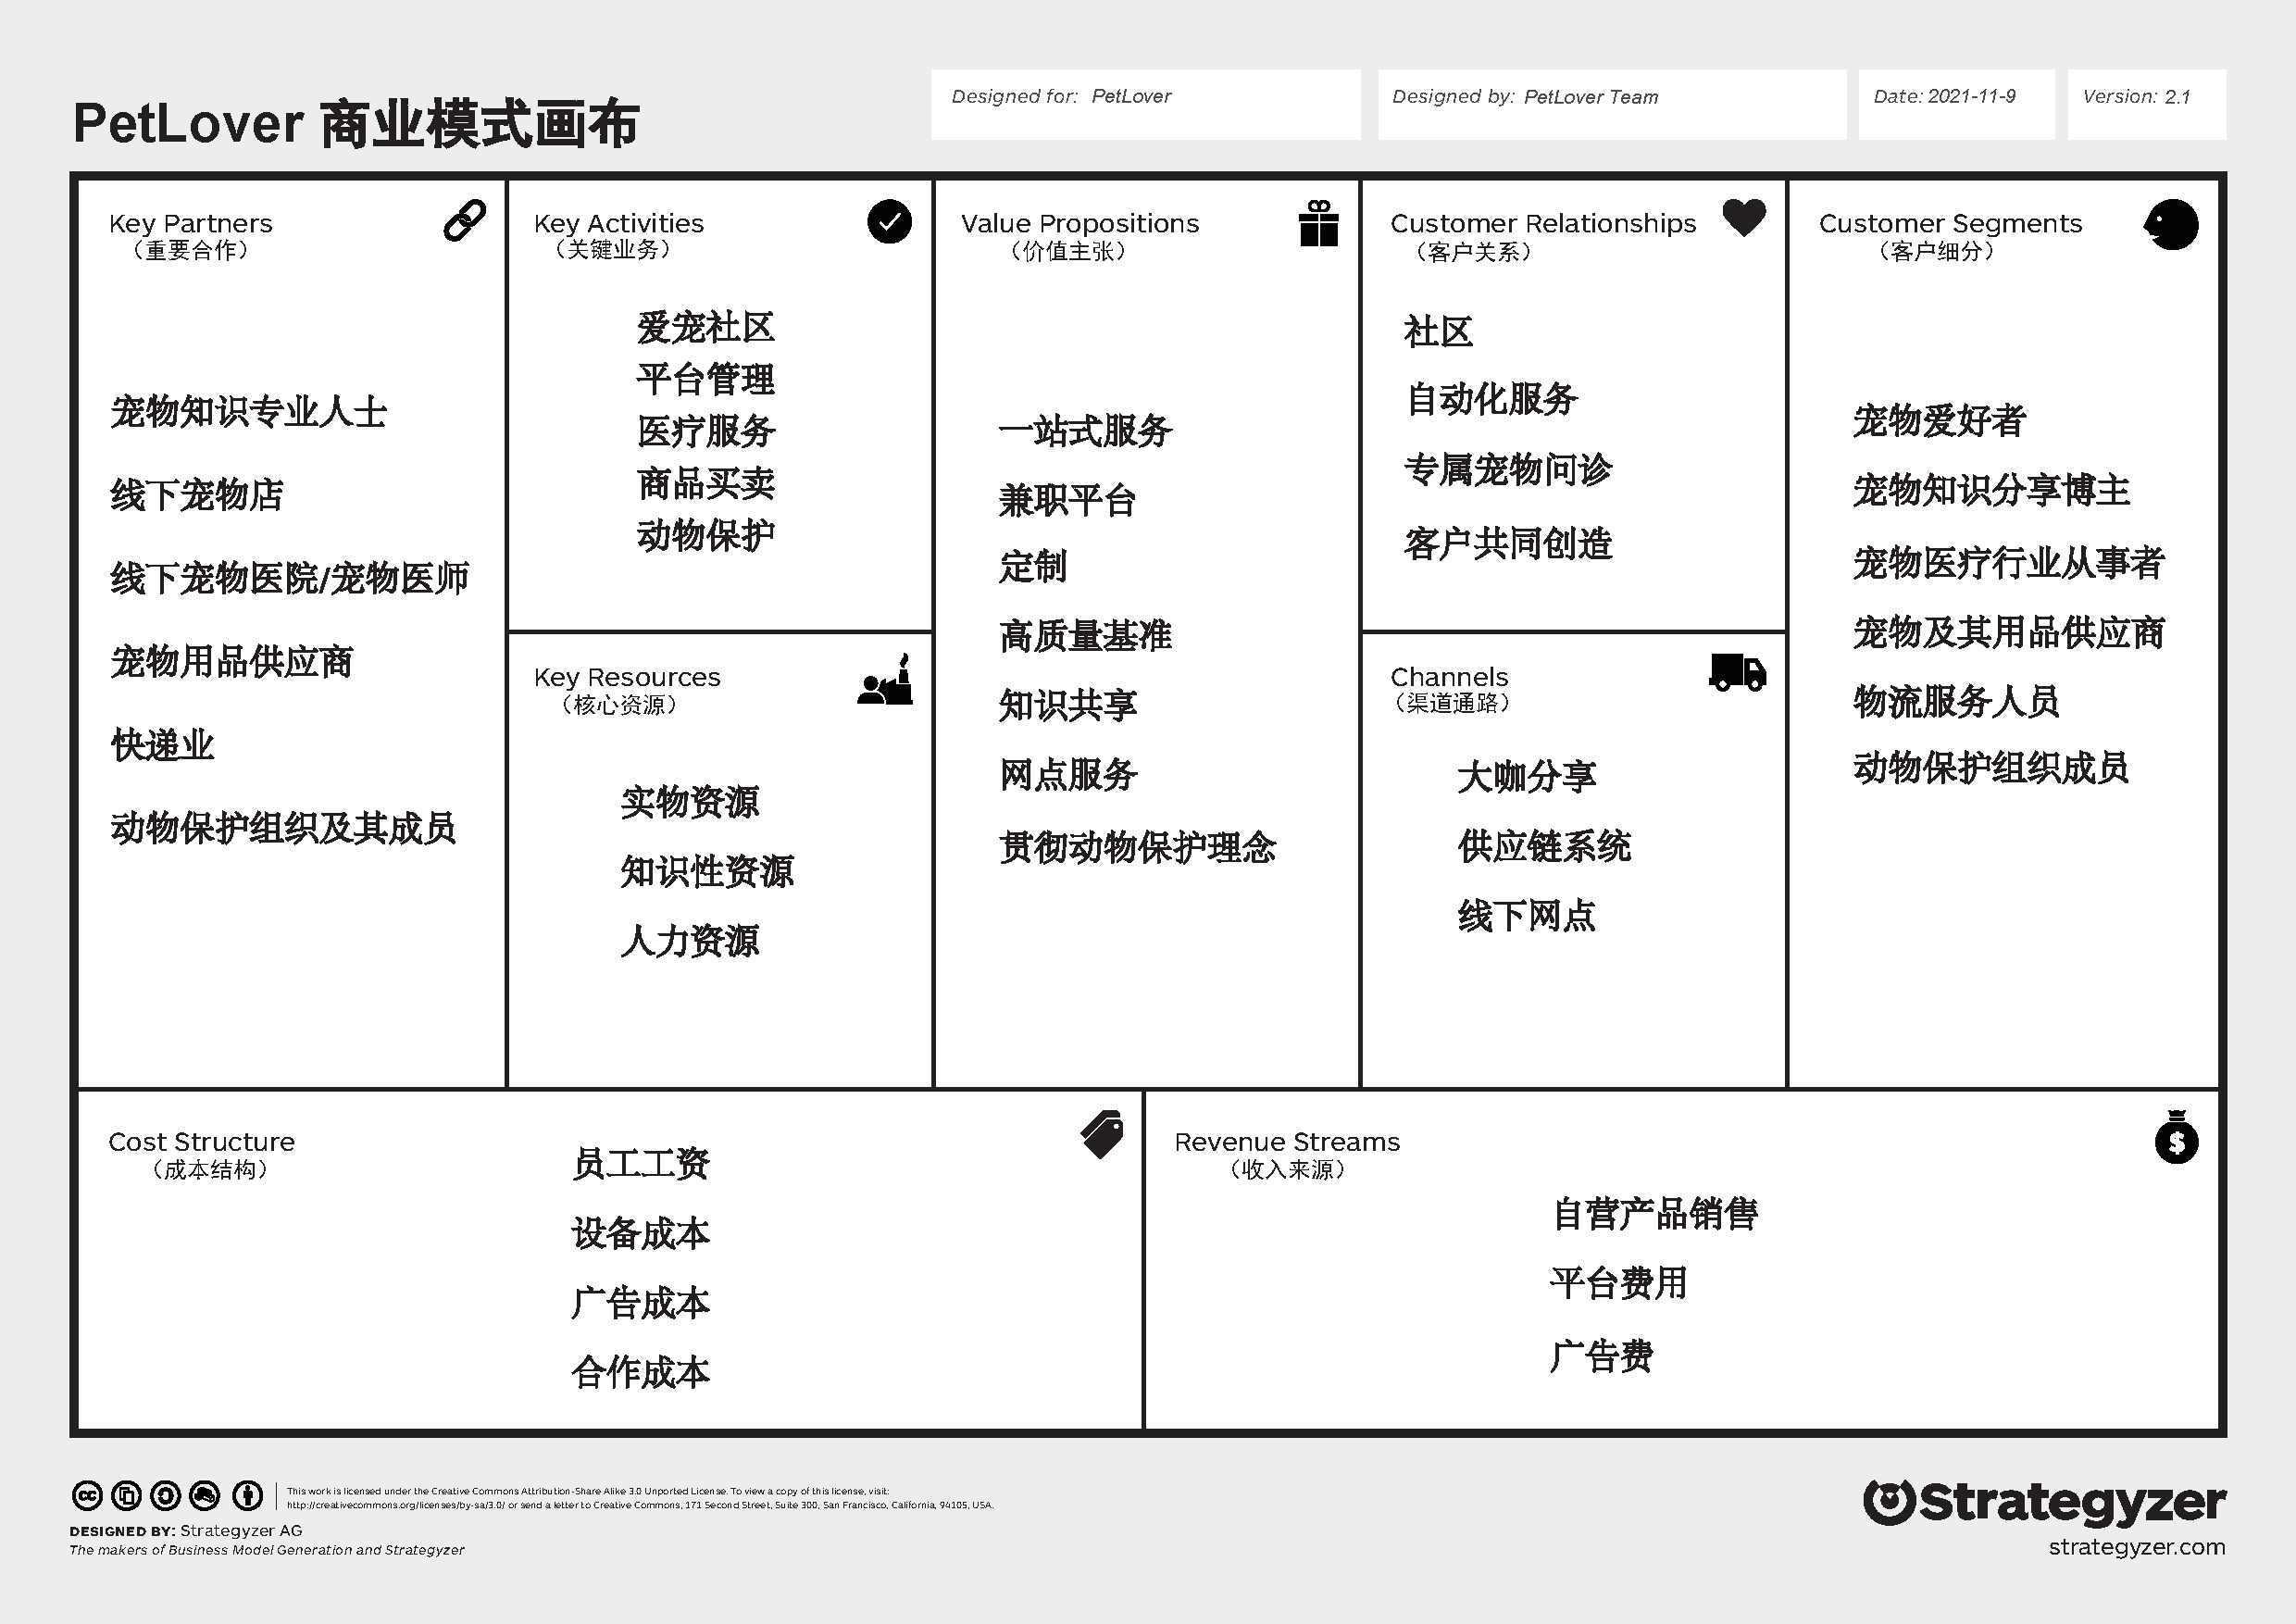
\includegraphics[scale=0.4]{改动后画布.pdf}
\end{center}

高亮处为新增要点,我们还基于蓝海战略删除了客户细分中的广告商、价值主张中的缩减用户成本,综合商业模式环境和评估删除了渠道通路中的专属服务、关键业务中的上门服务,另外我们对客户关系中的社区的描述进行了修改,将重要合作里的中国小动物保护组织和动物保护志愿者合并为一个要点,将客户细分里的动物保护志愿者改为动物保护组织成员。以下为我们新增和修改要点的描述:

\begin{enumerate}[label=\alph*.]
  \item 高质量基准(新增,价值主张):平台对社区内容和电商模块进行严格质量把关,社区论坛内容需要经过二级审核(审核人员审核和平台管理员抽查审核),尽可能使内容不含不良信息和垃圾广告等;电商模块与合作的商家与机构签订商品与服务质量保证协议,严格审核商品质量;平台内节制广告宣传,合理而正确地规划广告位,追求原生广告和创意广告。PetLover为用户提供可靠干净的社区环境。
  \item 知识共享(新增,价值主张):PetLover面向的用户往往需要解决宠物相关的问题,大部分养宠人士所掌握的知识不足以支持他们为宠物提供贴心的照顾,因此PetLover平台会邀请和吸引宠物知识专业人士和大咖入驻平台,分享他们关于宠物如不同宠物种类品性、宠物疾病表现等相关知识,同时我们主张"知识无门槛",因此平台对知识分享不会收取相关费用,但允许博主将知识设置为付费或免费,同时会提供创作激励。
  \item 网点服务(新增,价值主张):PetLover在各地加盟线下宠物服务网点,为辐射区域内的用户提供宠物的一系列服务,包括宠物生活服务、宠物医疗服务、商品配送服务等等,每个线下网点提供的服务范围可以有所不同,网点经营者可以根据需要自由选择。
  \item 宠物知识分享博主(新增,客户细分):平台吸引宠物专业人士或业余爱好者入驻平台,分享关于宠物如不同宠物种类品性、宠物疾病表现等相关知识,为其他用户答疑解惑,他们可以通过我们的创作激励获得收益,也可以无偿分享知识。
  \item 宠物知识专业人士(新增,重要合作):宠物专业人士为PetLover平台提供海量知识性资源,是保证宠物社区轮坛流量提升和活跃用户的重要力量,我们为宠物专业人士入驻者提供资金支持激励知识创作和分享,入驻者需要定期分享宠物相关知识。
  \item 社区(修改,客户关系):平台所服务的人群就是宠物相关从业者/爱好者,这些用户群体可以就宠物品种、宠物饲养、宠物诊疗等话题进行讨论,每位用户在相应的讨论中都可以发表自己的见解,共同建立氛围友善的宠物交流社区。同时社区内有共同爱好或交流甚欢的用户可以在同城宠物交友圈里建立私信或群聊交流。PetLover,让宠物爱好者不再孤独。
  \item 动物保护组织及其成员(修改,重要合作):为了秉持我们保护动物的价值主张,我们将在社区设立动物保护宣传板块,本平台将获得动物保护组织(如中国小动物协会)的许可和授权,吸引动物保护组织成员和自媒体入驻社区论坛,宣传动物保护思想,贯彻珍爱生命、倡导精神文明和发扬人道主义精神的理念。
  \item 动物保护组织成员(修改,客户细分):动物保护成员可以通过平台宣传呼吁保护动物,在论坛社区发布城市流浪动物的动态,对于一些可领养城市流浪动物发布流浪动物领养公告。
\end{enumerate}

新加入要点联系依赖如下:

\paragraph{1、高质量基准、广告费、广告成本、平台管理。}以高质量的宠物内容提升平台的知名度,以高质量的宠物在线问诊以及线下宠物服务奠定发展基础,平台在客户细分上剔除了广告商,削减了广告成本以及广告费。由于平台专营宠物相关用品,为了构建高质量宠物平台,广告的投放应该和宠物相关,且相关广告商为入驻的宠物用品电商,因此剔除;广告费为平台店铺推荐费用,为了向高质量基准靠拢,平台希望能够以入驻电商的质量进行推荐,减少了广告费收入。同时为了更加专注的营造平台,以内容取胜,削减了广告成本,不以热度作为平台发展核心。同时为了保证平台的高质量发展,必须要加强平台管理的关键业务。
\paragraph{2、贯彻动物保护理念、动物保护、动物保护组织及其成员、动物保护组织成员、合作成本}贯彻动物保护理念是平台的生命力所在,平台为了扩展动物保护这个关键业务的活动范围,将我们的动物保护志愿者的客户细分提升为动物保护组织成员,同时将中国小动物保护协会/动物保护志愿者的重要合作拓展为动物保护组织及其成员。同时强调了合作成本作为动物保护的经济支撑。
\paragraph{3、网点服务、线下网点、线下宠物店、线下宠物医院/宠物医师}平台希望能够线上整合零碎的线下宠物店和宠物医院,无论城市的发达与否,客户都能够享受到高质量的宠物服务,因此把线下网点的渠道通路进一步提升为我们新的价值主张——网点服务。同时增强了与线下宠物店、线下宠物医院/宠物医师的合作关系。
\paragraph{4、知识共享、知识性资源、宠物知识专业人士、爱宠社区、社区、客户共同创造、宠物知识分享博主、合作成本}为了打造高质量内容的社区,平台立足于知识共享的核心价值主张,增强了爱宠社区关键业务活动重要性,巩固社区的同时希望社区是每个在社区的爱宠人的社区,大家都能够为社区建设出力,因此强调了用户共同创造。在重要合作中,新引入了宠物知识专业人士作为我们的重要合作为建设知识共享社区出力,为平台创造知识性资源这个重要核心资源。同时增加了合作成本为建设高质量内容的社区作为经济基础。最后我们的客户细分拓展面向宠物知识分享博主,希望他们能利用社区知识资源的同时还可以回馈社区。

\subsection{商业画布详情}

最后,我们的商业模式画布如下

\begin{itemize}
  \item \textbf{关键业务}:PetLover平台业务面向为宠物相关,重点在于爱宠社区管理和商品买卖服务,具体分为爱宠社区、平台管理、医疗服务、商品买卖和动物保护。为宠物爱好者搭建一个可以交流宠物日常、养宠经验的社区论坛,用户可以通过文字、图片、短视频等媒介在社区中进行日常分享;我们注重平台管理,对社区内容和上坪管理进行严格质量把关,控制广告投放,保证用良好体验;提供宠物健康论坛及服务平台,通过宠物健康知识分享、宠物健康咨询、宠物线上问诊、宠物医疗线上预约、宠物药品配送等服务来帮助宠物主人保障爱宠的健康;联系各地区宠物或其用品商城使用该平台作为线上交易平台,宠物商品购物网点在全国形成宠物及用品供应网络;宣传动物保护思想是我们的附加关键业务,它可以升华平台底蕴的同时还可以吸引更多的平台客流量,提高平台的社会影响力,为后续平台的推广打基础。
  \item \textbf{价值主张}:PetLover平台价值主张力求贴合用户感受,围绕用户体验展开,具体位置一站式服务、兼职平台、定制化、高质量基准、知识共享、贯彻动物保护理念。实现用户的轻量化操作,避免宠物爱好者在其他各个服务平台反复切换,同时为知识型用户提供兼职的机会;通过推荐算法为不同用户群体定制不同的社区,尽可能满足用户需求,同时通过质量把关为用户提供可靠干净的社区环境;主张“知识共享”和“知识无门槛“,在”知识爆炸“的时代为用户提供有求必应的环境;在各地加盟线下宠物服务网点,为辐射区域内的用户提供宠物的一系列服务,让宠物饲养者生活更加方便;贯彻动物保护理念,提高社会影响力,这也是我们的企业文化。
  \item \textbf{客户细分}:PetLover平台主要为宠物爱好者提供服务,打造可靠、洁净、便捷的养宠环境。同时吸引宠物知识博主、宠物医疗行业从事者、宠物及其用品供应商、物流服务人员及动物保护组织成与平台合作,他们为平台提供实物资源、知识性资源、人力资源,为平台提供平台费用、广告费等收入,互惠互利,实现共赢。
  \item \textbf{客户关系}:顺应我们的价值主张,平台主要维护社区和客户共同创造的客户关系,以营造健康的爱宠社区,并产生源源不断的知识性资源;此外,平台还致力于提供专属宠物问诊的关系,以使有宠物问诊需求的用户和平台招募的专业宠物医师进行一对一交流,并进行后续的跟进问诊并给出针对性建议;平台通过有温度、有人情味的推荐算法为用户提供自动化服务,为用户推荐他们切实需要的。
  \item \textbf{渠道通路}:我们平台的渠道通路以大咖分享和线下网点为主,辅以供应链系统,形成联动营销模式,实现全渠道的跨界整合。首先,平台通过邀请爱宠明星、网红等大咖入驻,将宠物的饲养心得、宠物日常等高质量的原创“安利”内容以笔记的形式在社区发布,使得用户产生信任感与权威感,以达到吸引用户提高知名度的目的,做到产品运营、品牌营销、吸粉增粉三者合一。同时,平台与线下的宠物店、宠物用品店、宠物医院等达成合作,形成遍布各地的线下网点。在线下网点中,每一个消费者都可以成为品牌和口碑的传播者,最终转变为用户和忠实粉丝。此外,平台通过自营旗舰店、国内仓库和线下实体店形成供应链系统。平台提供的电商系统与供应链系统可以有机结合,实现评价-购买-传递-售后的一条龙增长。
  \item \textbf{重要合作}:我们的渠道通路和客户细分决定了我们的重要合作,保障平台完善的供应链系统、大咖分享、线下网点等渠道通路,需要我们与线下宠物店、宠物医院、快递行业和专业宠物知识分享博主进行长期密切的合作,为用户提供省心可靠的一站式服务;我们还与动物保护组织及成员进行合作,以贯彻动物保护理念,动物保护志愿者可以进行认证,并在爱宠社区中进行动物保护知识的宣传。
  \item \textbf{核心资源}:我们的平台主要是线上平台,知识性资源是平台的主要资源,主要由用户生产的资料组成,包括各种宠物饲养知识、宠物医师的科普文章等。同时,我们平台需要和线下宠物店、宠物医院、快递行业开展密切友好的合作,因此销售点管理系统、运输系统、线下网点都是我们重要的实物资源。此外,平台的软件开发团队、核心用户、知识分享博主等是我们重要的人力资源。
  \item \textbf{成本结构}:我们平台知识共享的价值主张决定了我们的成本以广告成本与合作成本为主。为了让平台拥有初始的精品笔记分享、常驻的宠物医师以及宠物店,来打造平台的原生社区环境,平台需要支付聘请宠物博主、宠物医师以及加盟宠物店的合作费;同时,平台初期需要大量的广告宣传来提高知名度,扩充基础个人用户量,维持日活跃用户流量。除了广告成本与合作成本,我们的成本还包括员工工资与设备成本。
  \item \textbf{收入来源}:基于网点服务的价值主张,平台支持第三方宠物店交易以及宠物医院问诊,从中收取平台费用,包括合作过程中收取的加盟费、服务过程中收取的交易手续费等。同时,基于一站式服务的价值主张,我们的平台支持宠物以及宠物用品交易,提供自营店与专卖店,掌握供应链,完善售后客服,提供一系列完整的消费服务,从中收取自营产品销售的利润。此外,为了便于宠物店与宠物用品店宣传,平台提供一些区域作为发布广告的场所,以及提供电商模块中的竞价排名,可以从中收取广告费用。
\end{itemize}
\end{document}